\documentclass{thesis}
\usepackage{graphicx}   % if you want to include graphics files
\usepackage[
    style=numeric,
    natbib=true,
    sorting=none
]{biblatex}
\usepackage{amsmath}
\usepackage{hyperref}
\usepackage{enumitem}
\usepackage{multirow}
\usepackage{adjustbox}
\usepackage{subcaption}

%\usepackage{draftwatermark}

\usepackage{tikz} % Required for drawing the watermark in the foreground
\usepackage{transparent} % Allows opacity so you can see figures underneath

% 1. Create a simple toggle for the watermark
\newif\ifDraftWatermark
\DraftWatermarkfalse % Default to OFF

% 2. Define the watermark content and position
\newcommand{\DrawWatermark}{%
  \begin{tikzpicture}[remember picture, overlay]
    \node[
      rotate=45,              % Angle
      scale=10,               % Size
      opacity=0.5,            % Transparency (0.1 = faint, 1.0 = solid)
      text=black!30,           % Color (light gray)
      align=center
    ] at (current page.center) {
        NOT FOR \\ REVIEW
      %\textbf{NOT FOR\\ REVIEW}   % Your Text
    };
  \end{tikzpicture}%
}

% 3. Hook into the "Foreground" layer of every shipout (page build)
\AddToHook{shipout/foreground}{%
  \ifDraftWatermark % Only draw if our toggle is ON
    \DrawWatermark
  \fi
}


%\usepackage{xcolor}                           
%\usepackage{listings}                         
                                              
% Colors for syntax highlighting              
%\definecolor{codegreen}{rgb}{0,0.6,0}         
%\definecolor{codegray}{rgb}{0.5,0.5,0.5}      
%\definecolor{codepurple}{rgb}{0.58,0,0.82}    
%\definecolor{backcolour}{rgb}{0.95,0.95,0.92} 
%\definecolor{stringcolor}{RGB}{42, 0, 255}    
%\definecolor{numbercolor}{RGB}{255, 0, 0}     
%\definecolor{keycolor}{RGB}{127, 0, 85}       
%                                              
%% General listing style                       
%\lstdefinestyle{mystyle}{                     
%    backgroundcolor=\color{backcolour},       
%    commentstyle=\color{codegreen},           
%    keywordstyle=\color{magenta},             
%    numberstyle=\tiny\color{codegray},        
%    stringstyle=\color{codepurple},           
%    basicstyle=\ttfamily\footnotesize,        
%    breakatwhitespace=false,                  
%    breaklines=true,                          
%    captionpos=b,                             
%    keepspaces=true,                          
%    numbers=left,                             
%    numbersep=5pt,                            
%    showspaces=false,                         
%    showstringspaces=false,                   
%    showtabs=false,                           
%    tabsize=2                                 
%}                                             
%\lstset{style=mystyle}                        
%                                              
%% JSON language definition                    
%\lstdefinelanguage[JSON]json{                 
%    keywords={true, false, null},             
%    keywordstyle=\color{keycolor},            
%    string=[s]{""}{""},                       
%    stringstyle=\color{stringcolor},          
%    numberstyle=\color{numbercolor},          
%    comment=[l]{//},                          
%    commentstyle=\color{gray}\ttfamily,       
%    morecomment=[s]{/*}{*/},                  
%    literate=                                 
%        *{0}{{{\color{numbercolor}0}}}{1}     
%         {1}{{{\color{numbercolor}1}}}{1}     
%         {2}{{{\color{numbercolor}2}}}{1}     
%         {3}{{{\color{numbercolor}3}}}{1}     
%         {4}{{{\color{numbercolor}4}}}{1}     
%         {5}{{{\color{numbercolor}5}}}{1}     
%         {6}{{{\color{numbercolor}6}}}{1}     
%         {7}{{{\color{numbercolor}7}}}{1}     
%         {8}{{{\color{numbercolor}8}}}{1}     
%         {9}{{{\color{numbercolor}9}}}{1}     
%}






\makeatletter
\newcommand{\lambdabar}{{\mathchoice
  {\smash@bar\textfont\displaystyle{0.25}{1.2}\lambda}
  {\smash@bar\textfont\textstyle{0.25}{1.2}\lambda}
  {\smash@bar\scriptfont\scriptstyle{0.25}{1.2}\lambda}
  {\smash@bar\scriptscriptfont\scriptscriptstyle{0.25}{1.2}\lambda}
}}
\newcommand{\smash@bar}[4]{%
  \smash{\rlap{\raisebox{-#3\fontdimen5#10}{$\m@th#2\mkern#4mu\mathchar'26$}}}%
}
\makeatother

\makeatletter
\newcommand{\saveequation}[2]{% #1 = label, #2 = math
  #2 \label{#1}
  \protected@write\@mainaux{}{\string\SAVEEQUATION{#1}{\unexpanded{\unexpanded{#2}}}}%
}
\newcommand{\SAVEEQUATION}[2]{%
  \global\@namedef{SAVEDEQUATION@#1}{#2}%
}
\newcommand{\repeatequation}[1]{%
  \ifcsname SAVEDEQUATION@#1\endcsname
    \@nameuse{SAVEDEQUATION@#1}\tag{\ref{#1}}%
  \else
    ?? \notag
  \fi
}
\makeatother


\addbibresource{bibliography.bib}

% Use the first command below if you want captions over 1 line indented.
% A side effect of this is to remove the use of bold for captions. 
% To restore bold, also include the second line below.
%\usepackage[hang]{caption}     % to indent subsequent lines of captions
%\renewcommand{\captionfont}{\bfseries} % only needed with caption package;
                                        %   otherwise bold is default)
                                        
%%%%%%%%%%%%%%%%%%%%  supply titlepage info  %%%%%%%%%%%%%%%%%%%%%
\thesistitle{\bf Determining Resonance Parameters of Self-Shielded Measurements in the Unresolved Resonance Region}        
\author{Alec William Golas}        
\degree{}
\department{Nuclear Engineering} % provide your area of study here; e.g.,
%  "Mechanical Engineering", "Nuclear Engineering", "Physics", etc.
\thadviser{Yaron Danon}
\signaturelines{5} 
\memberone{Dr. Wei Ji}        
\membertwo{Dr. Emily Lu}        
\memberthree{Dr. David Brown}
\memberfour{Dr. Devin Barry}
%\cothadviser{First co-adviser} %if needed
%\cocothadviser{Second co-adviser} % if needed
%  For a masters project use \projadviser instead of \thadviser, 
%  and \coprojadviser and \cocoprojadviser if needed. 
\submitdate{November 2025}        
%\copyrightyear{1685}  % if date omitted, current year is used. 
%%%%%%%%%%%%%%%%%%%%%   end titlepage info  %%%%%%%%%%%%%%%%%%%%%%
      
\begin{document} 
\titlepage             % Print titlepage   
%\copyrightpage        % optional         
\tableofcontents       % required 
\listoftables          % required if there are tables
\listoffigures         % required if there are figures


\chapter{Introduction}
\label{chap:introduction}
\section{Objective}
    This research project had two primary objectives. The first was to enable the determination of resonance parameters for the unresolved resonance region (URR) directly from self-shielded measurements. To accomplish this, the self-shielding code SESH\cite{sesh} was verified, validated, and integrated into the nuclear resonance parameter fitting code SAMMY\cite{sammy}, along with the development of a multi-isotope fitting capability not previously available in SAMMY's URR interface.

    The second objective was to apply these newly developed tools to produce a new evaluation of the URR for $^{90}$Zr and $^{91}$Zr. This evaluation leveraged both historical and newly available experimental data, including measurements on both enriched and natural zirconium samples, to improve the determination of average resonance parameters for these isotopes.


\section{Problem Description}

    In nuclear engineering, the neutron cross section can be divided into four energy regions: the thermal region, the resolved resonance region (RRR), the unresolved resonance region (URR), and the fast region. In the thermal region, cross sections generally follow a $1/v$ dependence and are well characterized. The resolved resonance region is where individual nuclear resonances can be experimentally resolved. The fast region is where the cross section is smooth. The unresolved resonance region is where resonances are too closely spaced to be resolved experimentally, leading to overlapping resonances that are observed as a continuous, fluctuating structure. This underlying resonance structure in the URR is accounted for in neutron transport codes by the use of probability tables. These probability tables are essentially a histogram of different possible cross section values for any given energy. The histograms which make up these probability tables are populated by simulating cross section resonances in the URR based on average resonance parameters and the parameters' known statistical distributions. NJOY\cite{njoy} is one such code that is responsible for generating these histograms from average resonance parameters. Accounting for resonance structure is essential for correctly modeling critical systems.





    Consider the IMF-10 Criticality Benchmark\cite{icsbep}, which is a 9\% enriched uranium cylindrical system with a depleted uranium reflector. Because uranium isotopes, particularly $^{238}$U, have a significant unresolved resonance region, this benchmark provides a clear demonstration of the importance of accounting for URR self-shielding in reactor calculations. This benchmark was modeled in the Monte Carlo neutron transport code MCNP\cite{mcnp} using cross sections generated from the ENDF/B-VIII.0 nuclear data library\cite{endf-8} and processed with NJOY. When probability tables are enabled, MCNP samples cross-section values at each collision in the URR from a probability table that captures the statistical distribution of cross sections due to unresolved resonance fluctuations. These probability tables are generated by NJOY from the average resonance parameters stored in the evaluated nuclear data file. When probability tables are disabled, MCNP instead uses only the smooth, energy-averaged cross section in the URR, which neglects the effect of resonance fluctuations entirely. To demonstrate the impact of this distinction, the benchmark was run with probability tables both enabled and disabled.

    \begin{table}[h!]
        \centering
        \caption{Impact of the URR on the IMF-10 Criticality Benchmark.}
        \begin{tabular}{|c  c  c|}
            \hline
            $k_{\text{eff}}$ (P-Tables On) & $k_{\text{eff}}$ (P-Tables Off) & $\Delta k$ (pcm) \\
            \hline
            $1.00274$ & $0.99806$ & $-468$ \\
            \hline
        \end{tabular}
        \label{tab:criticality-benchmark}
    \end{table}
    
    The results are given in \autoref{tab:criticality-benchmark}. Enabling the probability tables, which account for URR resonance fluctuations, resulted in a $\Delta k$ of approximately 468~pcm relative to the case where these fluctuations were neglected. This phenomenon is known as resonance self-shielding, which can be defined as the flux depression caused by strong resonances. This results in a reduction of the effective reaction rate, and therefore a reduction in the system's criticality.

    Accurate reactor calculations therefore require accurate average resonance parameters in the URR. These parameters are ultimately determined from experimental measurements, principally neutron transmission and capture yield experiments. In a transmission experiment, a beam of neutrons passes through a sample of material, and the fraction of neutrons that pass through without interacting is measured as a function of energy. The transmission is related to the total cross section via $T(E) = e^{-n\sigma(E)}$, where $n$ is the atomic thickness of the sample in atoms/barn. In practice, the energy resolution of the measurement is limited, meaning that the detector integrates over a finite energy bin. When this energy bin is wider than the spacing between individual resonances---as is inherently the case in the URR---the measured transmission represents an average over many resonance fluctuations within that bin. The key difficulty arises because the relationship between transmission and cross section is non-linear: the average of $e^{-n\sigma(E)}$ over an energy bin is not the same as $e^{-n\langle\sigma\rangle}$, where $\langle\sigma\rangle$ is the average cross section over that bin. This effect is known as resonance self-shielding, and it must be properly accounted for when extracting average resonance parameters from experimental data.

    Formally, this non-equivalence is stated as
    \begin{equation}
        \label{eq:self-shielding}
        \langle T (\sigma) \rangle \neq T(\langle \sigma \rangle)
    \end{equation}
    in which $\langle \cdot \rangle$ represents a quantity averaged over some energy region.
    
    This effect is illustrated in \autoref{fig:self-shielding-demo}, using \textsuperscript{181}Ta as an example. Consider a hypothetical single energy bin spanning from 2.2 to 2.38~keV, over which a transmission measurement is made on a sample with an atomic thickness of $n = 0.105$~atoms/barn. In reality, an experimenter measuring transmission in this energy bin would observe the average transmission
    \begin{equation}
        \label{eq:avg-transmission-def}
        \langle T \rangle = \frac{1}{\Delta E} \int_{\Delta E} e^{-n\sigma(E)}\, dE
    \end{equation}
    where $\Delta E = E_2 - E_1$ is the width of the energy bin and $\sigma(E)$ is the true energy-dependent cross section. This quantity is shown as the green line in \autoref{fig:self-shielding-demo}. Also shown is the finely resolved transmission $T(E) = e^{-n\sigma(E)}$ (blue line), which represents the transmission that would be observed if the energy resolution were infinitely fine; this quantity is not directly measurable in the URR, but is useful for illustration. Finally, the orange line shows $e^{-n\langle\sigma\rangle}$, the transmission calculated from the average cross section over the bin.
    
    It should be noted that in a real experiment, the measured average transmission also depends on the energy distribution of the incident neutron flux, $\phi(E)$, within the bin:
    \begin{equation}
        \label{eq:flux-weighted-transmission}
        \langle T \rangle_{\text{meas}} = \frac{\int_{\Delta E} \phi(E)\, e^{-n\sigma(E)}\, dE}{\int_{\Delta E} \phi(E)\, dE}
    \end{equation}
    For the purposes of this illustration, a uniform flux within the bin is assumed.

    \begin{figure}
        \centering
        \includegraphics[width=0.95\textwidth]{Introduction/Figures/ta181_transmission.pdf}
        \caption{Demonstration of Self-Shielding for \textsuperscript{181}Ta comparing the `True Transmission' (blue line), `Average Transmission' (green line), and `Transmission of Average Cross Section' (orange line).}
        \label{fig:self-shielding-demo}
    \end{figure}

    The central observation from \autoref{fig:self-shielding-demo} is that $\langle T \rangle > e^{-n\langle\sigma\rangle}$: the average transmission is always greater than the transmission of the average cross section. This discrepancy is the self-shielding effect, and it is what prevents a fitting code like SAMMY\cite{sammy} from being used directly with URR measurements without a correction for self-shielding.

    To summarize, the problem can be stated as follows:
    \begin{enumerate}
        \item The resonance structure in the URR cannot be ignored in modeling critical systems.
        \item Modeling the resonance structure in the URR requires accurate average resonance parameters.
        \item These parameters are extracted from transmission and capture experiments, which are subject to self-shielding in the URR.
    \end{enumerate}

    Therefore, a problem remains: how can an average measurement be expressed as a function of the average cross section? It wouldn't be sufficient to fit resonance parameters using the ``uncorrected'' cross-section, i.e.,
    \begin{equation}
        \overline{\sigma} = -\frac{1}{n} \ln{\langle T \rangle}
    \end{equation}
    as this value is heavily dependent on experimental conditions such as temperature and sample thickness, and does not account for self-shielding. The resonance parameters obtained from fitting $\overline{\sigma}$ would not accurately represent the true cross section.

    \begin{figure}[h]
        \centering
        \includegraphics[width=0.95\linewidth]{Implementation/Figures/OriginalWorkflow.pdf}
        \caption{Original Self-Shielding Correction Workflow for Fitting in URR}
        \label{fig:original-self-shielding-workflow}
    \end{figure}

    If resonance parameters which accurately describe the true average cross section are to be obtained, self-shielding must be accounted for. In order to do that, a correction factor is used, such that
    \begin{equation}
        \label{eq:self-shielded-transmission}
        \langle T \rangle = e^{-n \langle \sigma \rangle} C_T
    \end{equation}
    This `transmission correction factor', $C_T$, corrects for the self-shielding effect produced by the resonance fluctuations in the URR.

    This project integrated self-shielding correction factors directly into SAMMY, enabling the code to fit self-shielded URR transmission and capture yield measurements. Additionally, the capability to fit multiple isotope samples, such as self-shielded transmission and capture measurements of natural samples, was introduced: a feature not previously available in SAMMY's URR fitting. This new functionality significantly modernized SAMMY's URR fitting interface. This developed package was then applied to a new evaluation of the unresolved resonance region for Zr\textsuperscript{90} and Zr\textsuperscript{91}, utilizing natural datasets to improve the performance of the fit, which had been previously computationally prohibitive and reliant on manual, error-prone methods due to the lack of multi-isotope functionality.

\chapter{Statistical Theory of the Unresolved Resonance Region}
\label{chap:theory}
\section{Unresolved Resonance Region}
\label{sec:unresolved-resonance-region}

The Unresolved Resonance Region (URR) presents similar nuclear reaction phenomena as the Resolved Resonance Region (RRR); however, the crucial distinction lies in the experimental observability of individual resonances. In the URR, the resonances are too closely spaced in energy to be experimentally resolved, meaning that individual resonance parameters (e.g., resonance energies and widths) cannot be directly determined. This stands in contrast to the RRR, where the Single-Level Breit-Wigner (SLBW) approximation (or more complex multi-level formulations) can precisely describe the energy-dependent cross section based on discrete resonance parameters.

Because a complete set of individual resonances cannot be resolved, it becomes impractical and often impossible to calculate the "true" point-wise cross section in the URR. Therefore, instead of determining explicit resonance shapes, evaluators resort to calculating \textit{average} cross sections. These average cross sections are derived from statistical properties of the resonances, such as average level spacings and average resonance widths, rather than their individual values. This approach assumes that these parameters are sufficiently statistical and therefore accurately models the average cross section in the URR.

This formulation provides a convenient analytical form for the average total cross-section. However, it is missing a crucial element of the unresolved resonance region. The underlying statistical nature of the \textit{true} cross section in the unresolved resonance region exhibits significant rapid fluctuations around this analytical average cross section. These rapid fluctuations are responsible for resonant self-shielding. Resonant self-shielding significantly impacts transport equations, and must be accounted for to accurately model neutron transport. The following section characterizes the impact of cross section variance due to resonance fluctuations.

\section{Resonance Self Shielding}
\label{sec:resonance-self-shielding}
Resonance self-shielding is a phenomena which occurs when the resolution of a measurement is less than the level spacing between resonances. It can be summarized as the non-linear relationship between an observable quantity, i.e., transmission, and the total cross-section. Self-shielding is a consequence of the variance of the cross-section over some energy region. As the variance in the cross-section increases, the energy-averaged transmission increases relative to the transmission of the average cross-section,
\begin{equation}
    \label{eq:self-shielding-definition}
    \langle T \rangle > e^{-n \langle \sigma \rangle}
\end{equation}
in which the operator $\langle \cdot \rangle$ denotes an energy-averaged quantity,
\begin{equation}
    \label{eq:energy-average-operator}
    \langle \cdot \rangle = \frac{1}{E_{1} - E_{0}} \int_{E_{0}}^{E_{1}} \cdot dE
\end{equation}
The energy-averaged transmission, $\langle T \rangle$, is given by:
\begin{equation}
    \label{eq:energy-average-Transmission}
    \langle T \rangle = \langle e^{-n \sigma(E)} \rangle
\end{equation}
in which $\sigma(E)$ is the total cross-section as a function, and $n$ is the thickness of some material.

To demonstrate how the variance in the cross-section contributes to self-shielding, consider the Taylor-Series expansion of $\langle T \rangle$. The energy-differential transmission can be redefined in terms of the average cross-section over that energy bin, and the deviation of the energy-differential cross-section from the average:
\begin{equation}
    \left\langle e^{-n \sigma(E)} \right\rangle = \left\langle e^{-n \langle \sigma \rangle} e^{-n \left(\sigma(E) - \langle \sigma \rangle \right)} \right\rangle
\end{equation}

Because $\langle \sigma \rangle$ has to be constant over that energy region, that can be rearranged to:
\begin{equation}
    \label{eq:taylor-series-step}
    \left\langle e^{-n \sigma(E)} \right\rangle = e^{-n \langle \sigma \rangle} \left\langle e^{-n \left( \sigma(E) - \langle \sigma \rangle \right)} \right\rangle
\end{equation}
The second term in \autoref{eq:taylor-series-step} can be approximated using a Taylor expansion:
\begin{equation}
    e^{-n \left( \sigma(E) - \langle \sigma \rangle \right)} \approx 1 + n (\sigma(E) - \langle \sigma \rangle) + \frac{n^{2}}{2} (\sigma(E) - \langle \sigma \rangle)^2
\end{equation}
Taking the average of this approximation, and noting that $\langle \sigma(E) - \langle \sigma \rangle \rangle = 0$, we get:
\begin{equation}
    \left\langle e^{-n \left( \sigma(E) - \langle \sigma \rangle \right)} \right\rangle \approx 1 + \frac{n^{2}}{2} \langle (\sigma(E) - \langle \sigma \rangle)^2 \rangle = 1 + \frac{n^{2}}{2} \text{Var}(\sigma)
\end{equation}
This leads to the final approximation for $\langle T \rangle$:
\begin{equation}
    \label{eq:taylor-series-expansion}
    \langle T \rangle \approx e^{-n \langle \sigma \rangle} \left(1 + \frac{n^{2}}{2} \text{Var}(\sigma) \right) = e^{-n \langle \sigma \rangle} + \frac{n^{2}}{2} e^{-n \langle \sigma \rangle} \text{Var}(\sigma)
\end{equation}

Clearly, according to \autoref{eq:taylor-series-expansion}, as the variance in the cross-section increases, the self-shielding will increase. Consequently, by accounting for variance in the cross-section, the self-shielding will be accounted for.

\section{The Self-Shielding Correction Factor}
\label{sec:correction-factor}

The self-shielding correction factor is used to solve the inequality given in \autoref{eq:self-shielding-definition}. It is defined as:
\begin{equation}
    C_{T} = \frac{\langle e^{-n \sigma (E)} \rangle}{ e ^{- n \langle \sigma \rangle}}
\end{equation}

The experimental transmission obtained in the unresolved resonance region, $\langle T \rangle$, is given by:
\begin{equation}
    \label{eq:transmission}
    \left\langle T \right\rangle = \frac{1}{E_2 - E_1} \int_{E_1}^{E_2} e^{-n \sigma(E)}dE
\end{equation}
in which $\sigma(E)$ is the true cross section of the material. It is assumed that the energy bin is wide enough such that a statistically meaningful sample of resonances are captured.

In order to express the average transmission as a function of the average cross section:
\begin{equation}
    \label{eq:transmission-of-average}
    \left\langle T \right\rangle = \frac{1}{E_2 - E_1} \int_{E_1}^{E_2} e^{-n \left( \sigma(E) + \langle \sigma \rangle - \langle \sigma \rangle \right)}dE
\end{equation}
in which 
\begin{equation}
    \label{eq:energy-average-cross-section}
    \left\langle \sigma \right\rangle = \frac{1}{E_2 - E_1} \int_{E_1}^{E_2} \sigma(E) dE
\end{equation}
Therefore, the term defining the ``transmission of the average cross section'', $e^{-n \langle \sigma \rangle}$, can be removed, such that 
\begin{equation}
    \label{eq:corrected-average-transmission}
    \langle T \rangle = e^{-n \langle \sigma \rangle} C_T
\end{equation}
in which the term $C_T$ is known as the transmission correction factor, and is defined as:
\begin{equation}
    \label{eq:transmission-correction-factor}
    C_T = \frac{1}{E_2 - E_1} \int_{E_1}^{E_2} e^{-n \left( \sigma(E) - \langle \sigma \rangle \right)}dE
\end{equation}

In other words, the correction factor is the average deviation of the true cross section from the mean cross section over a given energy bin.
\begin{equation}
    \label{eq:ct-elegant-form}
    C_T = \left\langle e^{-n (\sigma - \langle \sigma \rangle)} \right\rangle
\end{equation}
or in a form that will be more useful in a later section (e.g. \autoref{sec:sesh}),
\begin{equation}
    \label{eq:ct-sesh-form}
    C_T = \frac{\langle e^{-n \sigma} \rangle}{ e^{-n \langle \sigma \rangle}}
\end{equation}


It should be noted that this is specifically the \textit{transmission} self-shielding correction factor. Other forms will be used later, but the end goal is the same: determine the average measurement as a function of the average cross section.

\section{Sampling Cross Sections from Average Parameters}
\label{sec:mc-sampling-from-average-parameters}

As previously stated in \autoref{sec:resonance-self-shielding}, in the Unresolved Resonance Region, individual resonances cannot be directly observed due to their close spacing. As such, only average resonance parameters can be obtained from measurements in the URR. While analytical equations, (e.g., \autoref{eq:hauser-feshbach-cross-section}), provide energy-averaged cross sections based on these average parameters, these analytical solutions intrinsically yield only the average behavior. They do not, however, directly provide the variance of the true, fluctuating energy-dependent cross section within the URR. The phenomenon of resonance self-shielding (discussed in \autoref{sec:resonance-self-shielding}) is directly dependent on this variance. However, this only discusses the determination of self-shielding from a known energy differential cross-section, which is not able to be observed.

Since the true energy-differential cross section in the URR is unknown, and its variance cannot be directly calculated from the average parameters alone, Monte Carlo methods provide the necessary means to address this challenge. By statistically sampling individual resonance parameters from their known probability distributions, Monte Carlo sampling allow for the generation of distribution of cross section "realizations" which agree with the average analytical cross section and account for the variance in cross section around said average. This section will detail how these fluctuating cross sections are determined from average parameters by leveraging the Single-Level Breit-Wigner (SLBW) equation, and sampling parameters from their respective statistical distributions.

\subsection{The Single-Level Breit-Wigner (SLBW) Equation for Cross Section Reconstruction}
\label{sec:slbw-for-sampling}

The Single-Level Breit-Wigner (SLBW) approximation\cite{t2}, typically used in the Resolved Resonance Region (RRR) for well-separated resonances, serves as the fundamental basis for reconstructing cross-section distributions from sampled resonance parameters in the URR. While more complex formalisms such as the R-Matrix theory are required to accurately model resonances in the RRR, the statistical nature of the URR allows for the use of the computationally simpler SLBW formula to generate cross-section realizations that are statistically consistent with the average parameters. For a given channel $c$, the total SLBW cross section\footnote{This isn't the \textit{total} total cross section as is generally referred to. Instead, it is the cross-section associated with forming a compound nucleus in a particular $J,\ell,\pi$ state, irrespective of the outgoing particle after the formation of that compound nucleus (neutron in the case of elastic scattering, $\gamma$-ray in the case of capture, etc). The incoming channel $c$ is used as shorthand for that $J,\ell,\pi$ state. The conventional \textit{total} total cross section is equivalent to summing over all possible channels.} is determined as a sum over resonances $r$ via:
\begin{equation}
    \label{eq:slbw}
    \sigma_c = \frac{ 4 \pi g_c}{k_c^2} 
        \left\{ \sin^2{\phi_c} + \sum_r \frac{\Gamma_{n,r,c}}{\Gamma_{tot,r,c}}
            \left( \psi_r \cos{2 \phi_{c}} + \chi_r \sin{2\phi_c}
            \right)
        \right\}
\end{equation}
The statistical spin factor, $g_c$ is defined as
\begin{equation}
    g_c = \frac{2J + 1}{2(2I + 1)}
\end{equation}
in which $I$ is the spin of the target nucleus, and $J$ is the total angular momentum (spin) of the resonance. The channel spin $s$ is formed by the coupling of the target spin $I$ and the neutron spin, while $J$ is formed by the coupling of $s$ and the orbital angular momentum $\ell$. $\phi_c$ is the hard-sphere scattering phase shift of a particular channel.

$\psi$ and $\chi$ are the Doppler broadened resonance profiles. Those are determined by using the Faddeeva function\cite{algo-916}, such that
\begin{equation}
    \label{eq:faddeeva}
    \psi + i\chi = \frac{\sqrt{\pi}}{2}\theta w \left(\frac{\theta x}{2}, \frac{\theta}{2} \right)
\end{equation}
in which $\theta$ is the Doppler width,
\begin{equation}
    \theta = \frac{\Gamma_{tot}}{\sqrt{\frac{4 \kappa T E}{A}}}
    \label{eq:doppler-width}
\end{equation}
$x$ is the resonance shape,
\begin{equation}
    x = \frac{2 (E - E_r)}{\Gamma_{tot}}
\end{equation}
and $w(\alpha,\beta)$ is defined as
\begin{equation}
    w(\alpha,\beta) = \frac{i}{\pi} \int_{-\infty}^{\infty} \frac{e^{-t^2}}{\alpha + i\beta - t}dt
\end{equation}
where the arguments to the Faddeeva function are $\alpha = \frac{\theta x}{2}$ and $\beta = \frac{\theta}{2}$.

The total microscopic cross section for a given nuclide at a specific energy is then determined by summing the contributions from all possible incoming channels $c$. Each channel corresponds to a unique set of quantum numbers (spin, orbital angular momentum, and parity) that contribute to the reaction. The other relevant reaction cross sections for a given channel can also be calculated from these parameters. The capture cross section:
\begin{equation}
    \sigma_{c,\gamma} =  \frac{ 4 \pi g_c}{k_c^2}  \sum_r \frac{\Gamma_{n,r,c} \Gamma_{\gamma,r,c}}{\Gamma_{r,tot}^2} \psi_r
\end{equation}
And the fission cross section is nearly identical:
\begin{equation}
    \sigma_{c,\gamma} =  \frac{ 4 \pi g_c}{k_c^2}  \sum_r \frac{\Gamma_{n,r,c} \Gamma_{f,r,c}}{\Gamma_{r,tot}^2} \psi_r
\end{equation}

The determination of all possible channel states will be elaborated in a later section. It is crucial to note that this SLBW formulation, as presented, presumes that the individual resonance parameters ($E_r$, $\Gamma_{n,r}$, and $\Gamma_{tot,r}$, for each resonance $r$) are precisely known. However, in the URR, these individual parameters are not experimentally resolved. Instead, only their \textit{average} values and statistical distributions are known. This discrepancy necessitates the use of statistical sampling techniques to generate instances of these resonance parameters from their average values and distributions, which then allows for the reconstruction of fluctuating cross sections using the SLBW equation.

\subsection{Sampling Cross-Sections from Average Parameters}
\label{sec:sampling-parameters}


The procedure for generating a statistical realization of the cross section over a given energy range involves several steps, iterated across different channels and multiple times to build a comprehensive distribution. For each given channel $c$, defined by a unique $(\ell, J, \pi)$ combination, a ladder of resonance energies is determined. This is done by sampling from the Wigner Distribution, in which
\begin{equation}
    \label{eq:wigner-distribution}
    P(s) = \frac{s\pi}{2 \langle D \rangle_c^2} e^{-\frac{\pi s^2}{4 \langle D \rangle_c^2}}
\end{equation}
where $\langle D \rangle_c$ is the average level spacing associated with that channel $c$, and $s$ is the sampled level spacing. This is used to produce a resonance ladder
\begin{equation}
    E_{c,r+1} = E_{c,r} + s
\end{equation}

The following step is to sample neutron widths for each channel and resonance energy.

\begin{equation}
    \label{eq:porter-thomas}
    \Gamma_{n,r,c} = P\left( \frac{\Gamma_{n,c}}{\langle \Gamma_{n,c}  \rangle}\right)\langle \Gamma_{n,c}  \rangle
\end{equation}
in which $\langle \Gamma_{n,c}  \rangle$ is the average neutron width for that channel, and $P\left( \Gamma_{n,c} / \langle \Gamma_{n,c}  \rangle \right)$ is the Porter-Thomas distribution, where:
\begin{equation}
    P(x) = \frac{e^{-x/2}}{\sqrt{2\pi x}}
\end{equation}

Once a neutron width for that channel is sampled, the total resonance width is determined. This is done as a sum over the neutron width plus the other possible channels, i.e., radiation width, fission width, and inelastic width:
\begin{equation}
    \Gamma_{tot,r,c} = \Gamma_{n,r,c} + \Gamma_{n',r,c} + \Gamma_{\gamma,r,c} + \Gamma_{f,r,c}
\end{equation}

These sampled parameters are processed via the steps described in \autoref{sec:slbw-for-sampling} to be input into \autoref{eq:slbw} and generate a cross section for that given channel $c$. This process is repeated for all possible channels to provides a single realization of the total cross section for a given set of average parameters:
\begin{equation}
    \sigma_{tot}^i = \sum_c \sigma_c
\end{equation}
Finally, this is repeated some $N$ number of realizations to produce a population of sampled cross sections, $\{ \sigma_{tot}^1, \sigma_{tot}^2, \ldots, \sigma_{tot}^{N} \}$. This set of sampled cross sections, if defined using accurate average parameters over some statistical number of resonances, will accurately reproduce the true variance in the energy-differential cross section over some energy bin.

This is the general procedure of how nuclear data processing codes (NJOY\cite{njoy}, FRENDY\cite{frendy}, AMPX\cite{scale2024manual}) simulate cross-section variance required to account for self-shielding in the URR. Self-shielding due to cross section variance from resonant fluctuations can therefore be accurately modeled strictly from average parameters.

Note, this only addresses total cross section. It does not mention partial cross sections, interpreting between parameters to be used in \autoref{eq:hauser-feshbach-cross-section} and \autoref{eq:slbw}, energy dependencies, or any approximations. Those details are implementation-specific, and will be discussed in subsequent chapters.


\chapter{Physics Model Implementation and Verification}
\label{chap:implementation}
This section describes the implementation of SESH into SAMMY as required for fitting resonance parameters to self-shielded URR measurements.

\section{URR Representation in SAMMY}

The average cross section in the URR is typically defined according to Hauser-Feshbach theory, which provides a framework for describing nuclear reactions proceeding through a compound nucleus when many channels are open and individual resonance effects are smeared out. The energy-averaged total cross section for an incoming channel $c$ can be expressed as:

\begin{equation}
    \label{eq:hauser-feshbach-cross-section}
    \langle \sigma_c \rangle =
    2 \pi \lambdabar_c^2 g_c \left\{
    1 - \frac{
            \cos{ ( 2 \phi_c)} \left[
                1 - \pi^2P_c^2 s_c^2 -  \left( P_c R_c^\infty \right)^2
            \right]
            + \sin{(2 \phi_c)} 2 P_c R_c^\infty
        }{
            \left( 1 + \pi P_c s_c \right)^2 + \left( P_c R_c^\infty \right)^2
    }
    \right\} \quad \text{}
\end{equation}
In this formulation, $\lambdabar$ is the reduced de Broglie wavelength for the neutron, $g_c$ is the statistical spin factor defined as $g_c = \frac{2J + 1}{2(2I + 1)}$ where $I$ is the spin of the target nucleus , and $\phi_c$ is the hard-sphere scattering phase shift for a particular channel. The form of $\phi_c$ depends on the orbital momentum $\ell$ and is a function of $\rho = \frac{a_c}{\lambdabar}$, where $a_c$ is the scattering radius of the target nucleus.

The parameters of significance to transmission self-shielding in the URR, which distinguish this average cross section from a simple energy average of RRR cross sections, are the distant level parameter $R^\infty_c$ and the strength function $\Tilde{S}_c$. Here, $P_c$ is the neutron penetrability, and $s_c$ is the pole strength, defined as $s_c = \Tilde{S}_c\lambdabar a_c \sqrt{E}/2$. The strength function $\Tilde{S}_c$ characterizes the average reduced width of resonances for a given orbital $\ell$.


\section{Converting from SAMMY Parameters to SESH Parameters}
    \subsection{Calculating Available Channels}

    As mentioned in the previous section, the relevant URR parameters are all given only as their $\ell$ basis. As a requirement for simulating resonances for calculating resonance self-shielding, these parameters need to be calculated according to $(J,\ell,\pi)$ rather than just $\ell$ dependencies.

    For an isotope with a ground-state spin $I$ interacting with a neutron (which has an intrinsic spin of $s_n = 1/2$), there are two possible channel spins: $s_{-} = I - 1/2$ and $s_{+} = I + 1/2$. This leads to two separate cases for the total angular momentum $J$: one for $s_{-}$ and one for $s_{+}$:
    \begin{align}
        J_{-} &= \left\{ \left|s_{-} - \ell\right|, \left|s_{-} - \ell\right| + 1, \cdots, s_{-} + \ell \right\}\\
        J_{+} &= \left\{ \left|s_{+} - \ell\right|, \left|s_{+} - \ell\right| + 1, \cdots, s_{+} + \ell \right\}
    \end{align}
    One common assumption is that spin-group parameters are assumed to be independent of parity, i.e., $(J, \ell, -1) = (J, \ell +1)$. As a consequence, only $J$ and $\ell$ need to be considered when calculating resonances. Instead, the important factor to consider is the degrees of freedom, or the multiplicity, $\mu$. If the same $J,\ell$ combination can be calculated from $s_{+}$ and $s_{-}$ channel spins, then $\mu_i = 2$. Otherwise, $\mu_i=1$.

    \begin{equation}
        \begin{array}{rrrrrrrr}
J_{-}: & \{ & \left|s_{-} - \ell\right|, & \left|s_{-} - \ell\right| + 1, & \dots, & s_{-} + \ell ~ & & \} \\
J_{+}: & \{ & & \left|s_{+} - \ell\right|, & \dots, & s_{+} + \ell-1, & s_{+} + \ell & \} \\[1em] \hline \\[-0.5em]
\mu_J: & \{& 1, & 2, & \dots, & 2, & 1 & \} \\
\end{array}
    \end{equation}

    \subsection{Converting from $R^\infty$ to $R'$}

    \subsection{Converting Inelastic Strength to Inelastic Widths from Channels}

\section{Improving Level Density Energy Dependency}

\section{Doppler Broadening Bug}
    The primary cause of the disagreement was determined to be the result of an error in the Doppler broadening subroutine that was originally present in SESH. In order to perform the Doppler broadening, the complex error function, also known as the Faddeeva function, is utilized. The issue was in the original algorithm, in cases where $\beta$ was less than 0.01. Recall that
    \begin{equation}
        w(\alpha,\beta) = \frac{i}{\pi} \int_{-\infty}^{\infty} \frac{e^{-t^2}}{\alpha + i\beta - t}dt
    \end{equation}
    and
    \begin{equation}
        \beta = \frac{\theta}{2} = \frac{\Gamma_{tot}}{4\sqrt{\frac{ \kappa T E}{A}}}
        \label{eq:doppler-beta}
    \end{equation}

    In instances where $\beta \leq 0.01$, the algorithm would incorrectly return the 0 Kelvin value for the $\psi$ parameter, shown in \autoref{fig:beta-error}.
    \begin{figure}
        \centering
        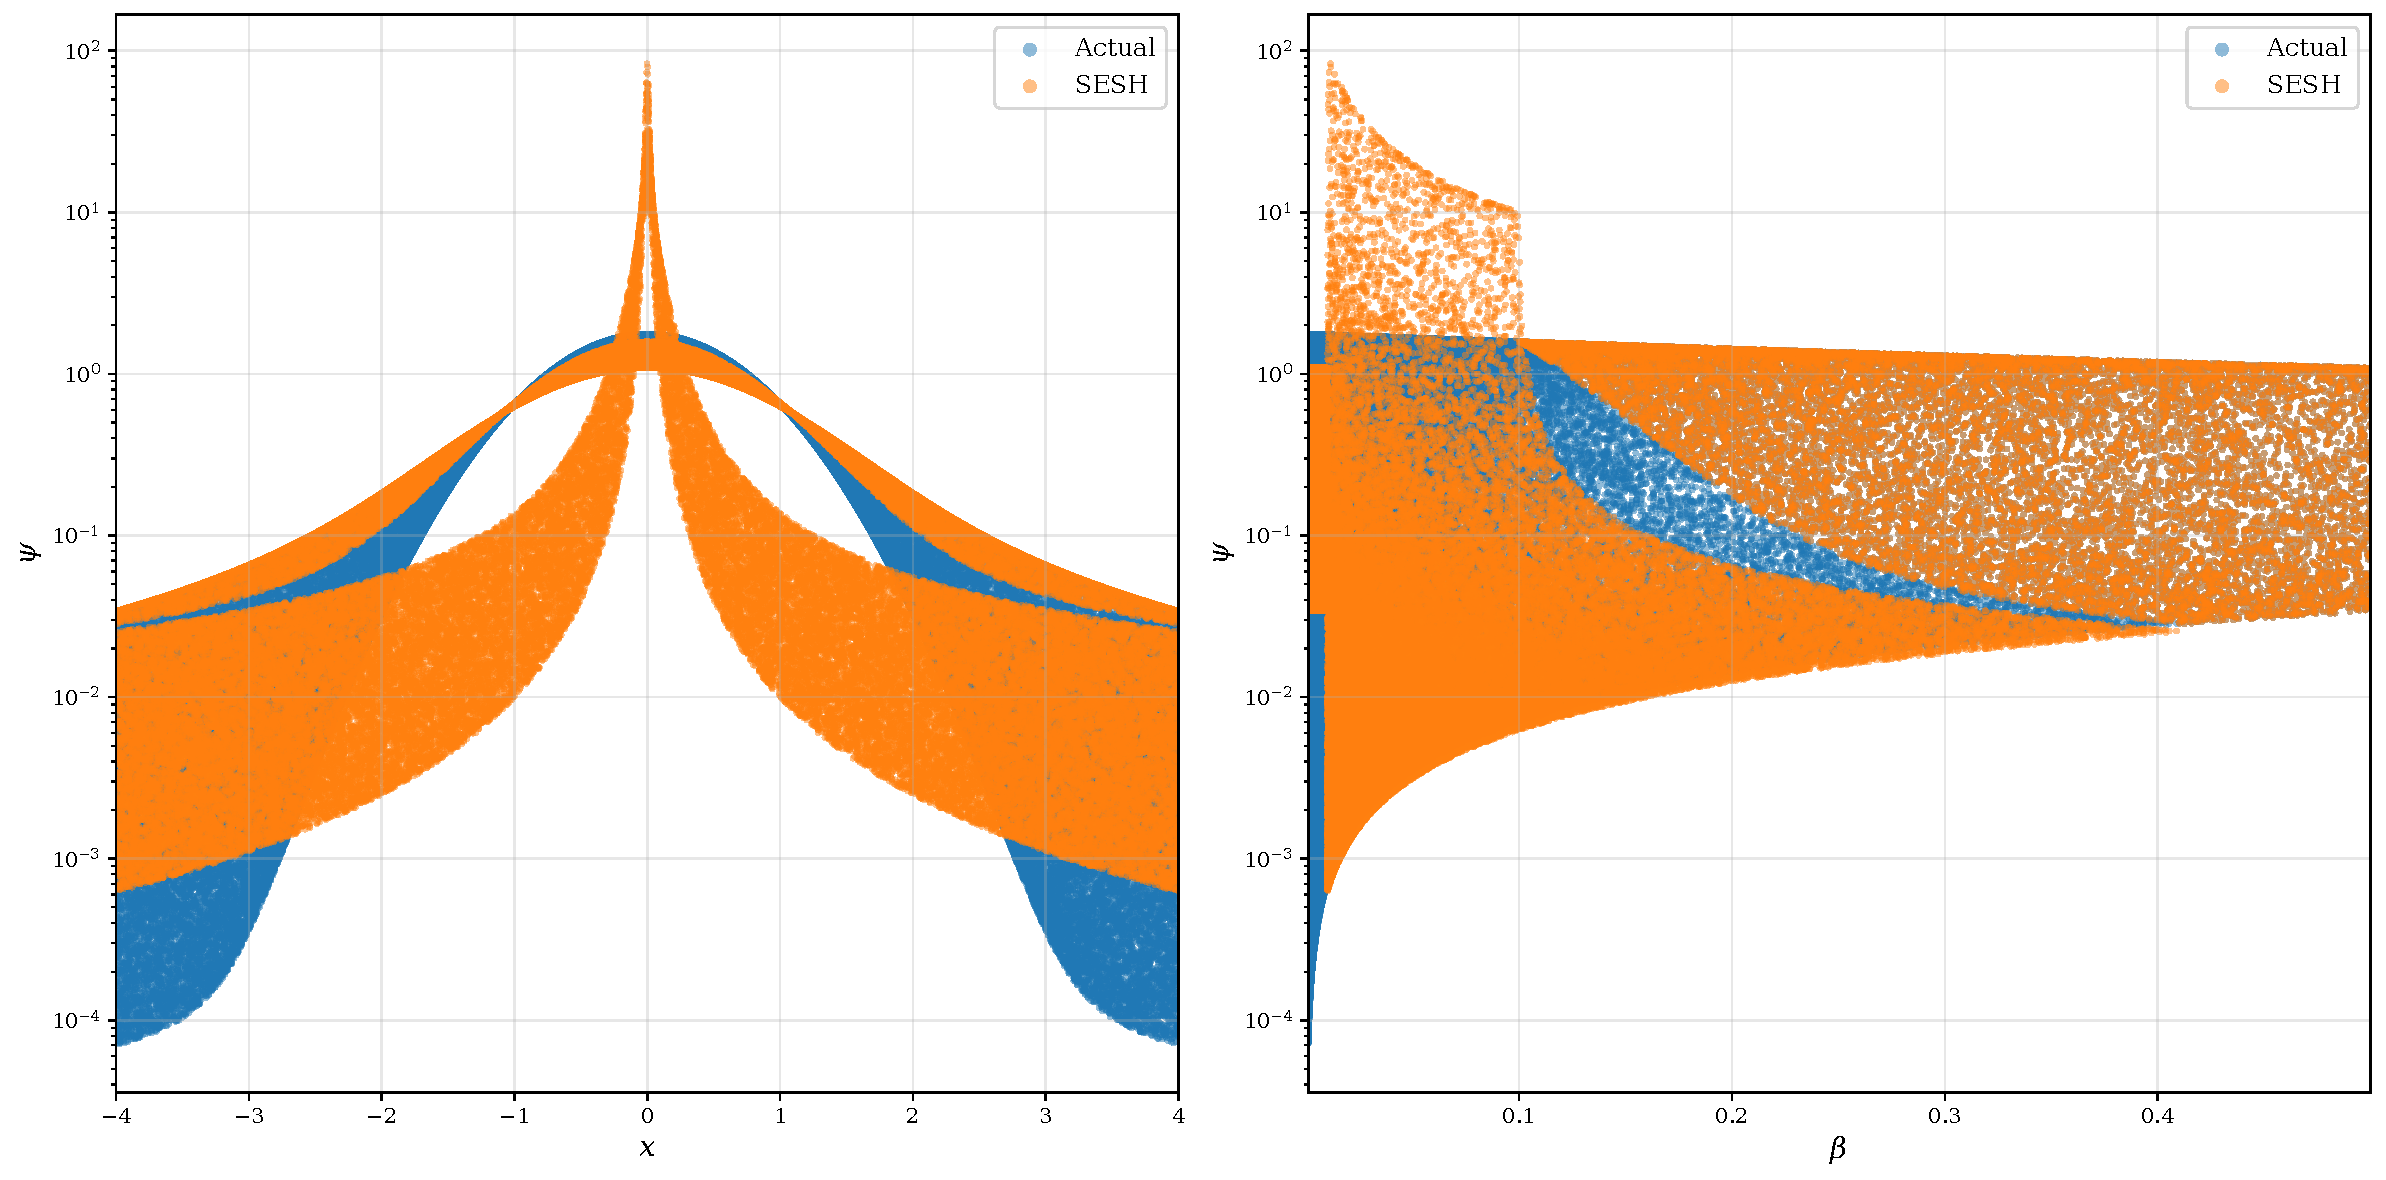
\includegraphics[width=0.95\linewidth]{Implementation/Figures/beta-error.png}
        \caption{Comparing results of SESH's Faddeeva function output with what the Faddeeva function actually calculates given the same inputs.}
        \label{fig:beta-error}
    \end{figure}
    
    One significant effect of this bug is due to the inverse relationship between $\beta$ and energy, shown in \autoref{eq:doppler-beta}. As the energy of the incident neutron increases, the probability of $\beta$ being sampled as less than 0.01 increases. Consequently, as energy increases, the probability of the 0 Kelvin cross section being returned also increased.

\section{Energy Deposition Improvement}
    Originally in SESH, there was a very simple approximation for sampling what energy an interaction occurred at. It was assumed that every neutron lost the average scattering energy per collision, independent of scattering angle, i.e.,
    \begin{equation}
        E' = E \left[ 1 - \frac{2A}{\left( 1 + A \right)^2} \right]
    \end{equation}
    for all post-collision neutrons. This enabled all of the energy dependent parameters that did not get sampled using the Monte Carlo method to be pre-calculated efficiently. However, it was assumed this would be an insufficient approximation for thick samples in which many collisions were expected.
    
    This was substituted with an angle-dependent energy sampling procedure. The scattering angle of each post collision neutron would be sampled assuming an isotropic scattering distribution, and the post collision energy would be calculated as a function of the scattering angle,
    \begin{equation}
        E' = E \frac{A^2 + 2 A \mu_c + 1}{\left( A + 1 \right)^2}
    \end{equation}
    in which
    \begin{equation}
        \mu_c = \cos\phi_c
    \end{equation}
    where $\phi_c$ is the exit angle of the post-collision neutron in the center-of-mass system.
    \begin{figure}
        \centering
        \includegraphics[width=0.95\linewidth]{Implementation/Figures/multiple_scattering.png}
        \caption{Distribution of neutrons after each collision using the old SESH post-collision energy sampling method and the new angle-dependent sampling in a 12mm \textsuperscript{181}Ta sample at 3keV initial incident energy.}
        \label{fig:multiple-scattering}
    \end{figure}

\chapter{Monotopic Transmission Correction}
\label{chap:transmission-correction}
This chapter details and validates the procedure for calculating the theoretical average transmission to accurately fit parameters to self-shielded transmission measurements in the URR\cite{Bahran2015}. As shown in \autoref{sec:resonance-self-shielding}, the theoretical average transmission can be calculated as the product of the transmission of the average cross section, $e^{-n\langle \sigma \rangle}$, and a transmission correction factor $C_T$. SESH uses Monte Carlo integration in order to determine these energy-averaged quantities\cite{sesh}.

SESH is used here as the transport engine that computes the self-shielding transmission correction factor $C_T$, while SAMMY performs the parameter fitting. The goal of this chapter is to validate that $C_T$ is calculated correctly and that applying it within SAMMY leads to consistent transmission predictions and stable fits.
\section{Transmission Correction for a Mono-Isotopic Sample}
\label{sec:tc-monotopic}

The calculation of the transmission correction factor is centered around a Monte Carlo simulation that generates a statistical population of cross-section realizations. This process, described in detail in Chapters \ref{chap:theory} and \ref{chap:implementation}, simulates the inherent fluctuations of the cross-section in the URR. For each Monte Carlo history, a ``resonance ladder'' is constructed for each channel by sampling resonance widths from the Porter-Thomas\cite{Porter1956} distribution and level spacings from a Wigner distribution\cite{Wigner1951}. These stochastically generated parameters are then used within the SLBW formalism\cite{Lane1958} to produce a single realization of the total microscopic cross-section, $\sigma_i$.

For each sampled cross-section, a corresponding transmission value is calculated, $T_{i} = e^{-n\sigma_{i}}$, where $n$ is the sample thickness. By repeating this for a large number of histories, a set of sampled cross-sections $\left\{ \sigma_{1}, ..., \sigma_{N} \right\}$ and a corresponding set of transmissions $\left\{ T_{1}, ..., T_{N}\right\}$ are obtained. From these sets, their respective averages are computed:
\begin{equation}
    \langle \sigma \rangle = \frac{1}{N} \sum_{i=1}^{N} \sigma_{i}
\end{equation}
and
\begin{equation}
    \langle T \rangle = \frac{1}{N} \sum_{i=1}^{N} T_{i}
\end{equation}

From these averages, the correction factor defined in \autoref{sec:resonance-self-shielding} can be approximated as:
\begin{equation}
    C_T \approx \frac{\langle T \rangle}{e^{-n\langle \sigma \rangle}}
\label{eq:CT_mc}
\end{equation}

The accuracy of this method will be validated using $^{181}$Ta, for which a recent evaluation provides new resonance parameters\cite{Brown2024}. The validation is twofold. First, the theoretical model is compared against MCNP simulations to provide a detailed characterization of its performance. As the MCNP model utilizes the exact best-fit parameters from the recent $^{181}$Ta evaluation, it serves as an useful reference case to investigate the effects of physical parameters such as sample thickness and temperature. Second, the calculated average transmission is compared against the experimental data that was used in the evaluation. This comparison serves to validate the theoretical model's overall performance for a single sample thickness, serving as a final integration test for SESH’s theoretical self-shielded transmission calculation.

\section{Verification of the Correction Factor Model}
Before integrating the transmission correction into the fitting procedure, it is essential to verify that SESH accurately calculates the correction factor itself. The verification was performed by comparing the results from SESH to those from a high-fidelity model of the experiment constructed using MCNP \cite{mcnp}. This MCNP model serves as a computational benchmark\cite{Humbert2014}, providing a a high-fidelity reference against which the statistical methods in SESH can be compared. Three key physical parameters that could influence the correction factor were investigated: the number of external resonance pairs used in the calculation, the physical thickness of the sample, and the temperature of the sample.

\subsection{MCNP Reference Model}
\label{ssec:mcnp-benchmark-model}

MCNP is used here as a transport reference: both MCNP and SAMMY/SESH use the same evaluated nuclear data, so the comparison primarily tests the correction method and its implementation rather than differences in input cross sections.
The MCNP model was configured to simulate neutron transmission through a $^{181}$Ta sample. The cross-section data for the simulation was prepared from the ENDF/B-VIII.1 evaluation \cite{endf-manual} and processed into a pointwise format using NJOY \cite{njoy}. By using the exact, finely-resolved cross sections from a formal evaluation, the MCNP simulation can directly calculate the true average transmission, $\langle T \rangle$, and the transmission of the average cross section, $e^{-n\langle\sigma\rangle}$, over a given energy group. The benchmark correction factor is then calculated as:
\begin{equation}
    C_{T, \text{MCNP}} = \frac{\langle T \rangle_{\text{P-Table=ON}}}{\langle T \rangle_{\text{P-Table=OFF}}}
\end{equation}
This provides an ideal reference value, free from the statistical approximations inherent to the SESH methodology, against which SESH's calculations can be validated.

\subsection{Monte Carlo Convergence}
\label{ssec:mc-convergence}

The preceding subsections validated the accuracy of the SESH correction factor against an MCNP benchmark, but the Monte Carlo procedure introduces a separate concern: statistical precision. Because $C_T$ is estimated from a finite sample of resonance ladder realizations, each evaluation carries a random fluctuation whose magnitude depends on both the number of histories $N$ and the physical conditions of the calculation. In a standalone comparison to data this fluctuation simply widens the scatter in the theoretical prediction. In the context of iterative fitting, however, an imprecise $C_T$ corrupts the derivative information used by the Bayesian update, causing the fit to oscillate around the minimum rather than converge smoothly.

To characterize the convergence behavior, the correction factor was computed for a 4~mm $^{181}$Ta sample at 300~K using four external resonance pairs at three representative energies spanning the URR: 5~keV, where self-shielding is strongest ($C_T \approx 1.043$); 20~keV, where the correction is moderate ($C_T \approx 1.006$); and 80~keV, where it is negligible ($C_T \approx 1.0005$). At each energy, the number of Monte Carlo histories was varied from $N = 25$ to $N = 100{,}000$, with 30 independent trials performed at each value of $N$ to estimate the standard deviation of the $C_T$ estimator.

\autoref{fig:ct-convergence-means} shows convergence of the computed correction factor as a function of $N$ at each energy. The mean value is stable across all $N$, confirming that the Monte Carlo estimator is unbiased. The error bars contract monotonically with increasing $N$, and the effect is most pronounced at 5~keV where the cross-section fluctuations are largest. At 80~keV, where the level density is high and individual resonances overlap strongly, even $N = 25$ histories produce a correction factor that is effectively converged.

The convergence rate is quantified more precisely in \autoref{fig:ct-convergence-precision}, which plots the relative standard deviation of $C_T$ against $N$. All three energies follow the expected $1/\sqrt{N}$ scaling of a Monte Carlo estimator, confirming that the variance arises from the stochastic sampling of resonance ladders and not from any systematic instability in the algorithm. The vertical separation between the curves reflects the magnitude of the self-shielding correction: larger corrections produce wider cross-section distributions, which require more histories to average precisely.

For the purpose of evaluating resonance parameters, the precision requirement on $C_T$ is more stringent than might be suggested by the correction factor alone. During fitting, SAMMY updates the average resonance parameters iteratively, with each step relying on the partial derivatives of the theoretical transmission with respect to the fitted quantities. When $C_T$ carries excessive statistical noise, these derivatives are contaminated, and the fit oscillates near the minimum rather than converging to it. In practice, this manifests as a final $\chi^2$ that fluctuates between iterations without settling, particularly for the strength functions whose effect on $C_T$ is small but physically meaningful. Empirically, stable convergence of the fitting procedure requires the relative precision on $C_T$ to be well below the sensitivity of the transmission to a single parameter step, which for typical URR evaluations corresponds to a relative standard deviation on the order of 0.1\% or better.

From \autoref{fig:ct-convergence-precision}, this threshold is reached at approximately $N = 50{,}000$ for the most heavily self-shielded case at 5~keV, where the relative standard deviation falls to 0.07\%. At 20~keV the same precision is achieved near $N = 10{,}000$, and at 80~keV it is reached with only a few hundred histories. In general, the required number of histories scales with the magnitude of the self-shielding correction: thicker samples of isotopes with wider resonance-width distributions and lower level densities will require more histories to achieve the same statistical precision. For the evaluations presented in \autoref{chap:evaluation}, $N = 50{,}000$ histories were used at all energies to ensure that the Monte Carlo noise in $C_T$ does not limit the fitting precision.

\begin{figure}[H]
    \centering
    \includegraphics[width=\textwidth]{Transmission Correction/Figures/ct_convergence_means.pdf}
    \caption{Convergence of the transmission correction factor for a 4~mm $^{181}$Ta sample at 300~K at three representative URR energies. Each point is the mean of 30 independent calculations; error bars show $\pm 1\sigma$. The dashed lines indicate the converged value at $N = 100{,}000$. The mean is unbiased at all $N$; only the statistical spread decreases with increasing history count.}
    \label{fig:ct-convergence-means}
\end{figure}

\begin{figure}[H]
    \centering
    \includegraphics[width=0.75\textwidth]{Transmission Correction/Figures/ct_convergence_precision.pdf}
    \caption{Relative standard deviation of the correction factor as a function of the number of Monte Carlo histories. The dashed line shows the expected $1/\sqrt{N}$ scaling. At 5~keV, where self-shielding is strongest, approximately $50{,}000$ histories are needed to reduce the relative uncertainty below 0.1\%. At higher energies where the correction is smaller, fewer histories suffice.}
    \label{fig:ct-convergence-precision}
\end{figure}

\subsection{Influence of External Resonance Pairs}
\label{ssec:resonance-pairs}

The Monte Carlo procedure in SESH constructs a set of resonance ladders within each energy bin by sampling level spacings and widths from their respective statistical distributions. In practice, the cross section at any point within the bin is not determined solely by the resonances inside it --- the tails of nearby resonances outside the bin also contribute. The question is how many of these external resonances need to be included to produce a statistically representative sample of the cross-section fluctuations.

When resonance widths are much larger than the mean level spacing ($\Gamma \gg D$), the cross section at a given energy is the incoherent sum of many overlapping resonance contributions, and the fine details of any individual resonance placement become unimportant\cite{ERICSON1963390}. In this regime, even a modest number of external resonances captures the essential behavior. However, $\Gamma/D$ is not uniformly large across the URR. At lower energies where level densities are smaller and resonances are more isolated, the cross section within a bin can be sensitive to whether a particular external resonance happens to sit just outside the bin edge. Monahan and Elwyn\cite{MONAHAN1967683} showed that fluctuations in the averaged compound cross section depend on both the width and spacing distributions, meaning that truncating the resonance ladder too aggressively can bias the sampled cross-section distribution and, in turn, the correction factor.

The SESH code addresses this by allowing the user to specify a number of external resonance pairs: resonances placed above and below the bin boundaries spaced by sampling from the Wigner Distribution\cite{Wigner1951}. Adding more pairs extends the sampled ladder further from the bin edges, ensuring that the tails of distant resonances are properly included in the cross-section calculation. To quantify the impact of this setting, the correction factor was calculated for a 4~mm $^{181}$Ta sample at 300~K using one through four external resonance pairs.

The results, shown in \autoref{fig:tc-resonance-pairs}, demonstrate that the inclusion of external resonance pairs has a slight but noticeable influence on the calculated correction factor. As more pairs are added, the SESH calculation converges toward the MCNP benchmark value. The effect is most visible at lower energies where the resonances are less overlapping and the bin-edge truncation matters more. By four external pairs the improvement saturates, and additional pairs produce no further change within the statistical precision of the calculation. For the remainder of this work, four external resonance pairs were used in all SESH calculations.

\begin{figure}[H]
    \centering
    \begin{subfigure}[b]{0.48\textwidth}
        \centering
        \includegraphics[width=\textwidth]{Transmission Correction/Figures/resonancepair_CT.pdf}
        \caption{SESH correction factor compared to MCNP (solid black line) for increasing numbers of external resonance pairs.}
        \label{fig:tc-resonance-pairs-data}
    \end{subfigure}
    \hfill
    \begin{subfigure}[b]{0.48\textwidth}
        \centering
        \includegraphics[width=\textwidth]{Transmission Correction/Figures/resonancepair_convergence.pdf}
        \caption{Convergence of $C_T$ toward the MCNP reference (dotted lines) as a function of the number of external pairs at selected energies.}
        \label{fig:tc-resonance-pairs-convergence}
    \end{subfigure}
    \caption{Effect of external resonance pairs on the transmission correction factor for a 4~mm $^{181}$Ta sample at 300~K. The correction converges by approximately four external pairs at all energies, with the effect most pronounced at lower energies where resonance overlap is weakest.}
    \label{fig:tc-resonance-pairs}
\end{figure}


\subsection{Sample Thickness Dependence}
\label{ssec:thickness}

Of the parameters investigated in this chapter, the sample thickness exerts the strongest influence on the transmission correction factor. This sensitivity follows directly from the physics of self-shielding: a thicker sample amplifies the nonlinear relationship between the cross-section fluctuations and the transmitted intensity. As presented in \autoref{eq:taylor-series-expansion},  the correction factor depends on the cross-section variance as $C_T \approx 1 + \frac{1}{2}n^2 \mathrm{Var}(\sigma)$, where $n$ is the sample thickness in atoms per barn. For thin samples the quadratic term is small and $C_T$ remains close to unity. But as $n$ increases the correction grows rapidly and the shape of the cross-section distribution become increasingly important.

To characterize this behavior and determine the range of applicability for SESH, the correction factor was computed for 2~mm, 4~mm, 8~mm, and 12~mm samples of $^{181}$Ta at 300~K and compared against the MCNP benchmark. The results are shown in \autoref{fig:tc-thickness}. For the thinner samples (2--4~mm), the agreement between SESH and MCNP is excellent, with relative errors below 0.1\%. For the thicker samples (8--12~mm), a systematic positive bias emerges in which SESH predicts a larger correction factor than MCNP, with the disagreement growing at lower energies where self-shielding is strongest.

\begin{figure}[H]
    \centering
    \begin{subfigure}[b]{0.48\textwidth}
        \centering
        \includegraphics[width=\textwidth]{Transmission Correction/Figures/thickness_CT.pdf}
        \caption{SESH correction factor (solid lines) compared to MCNP (open circles) for each sample thickness.}
        \label{fig:tc-thickness-data}
    \end{subfigure}
    \hfill
    \begin{subfigure}[b]{0.48\textwidth}
        \centering
        \includegraphics[width=\textwidth]{Transmission Correction/Figures/thickness_error.pdf}
        \caption{Relative deviation of SESH from MCNP as a function of incident energy, showing increasing disagreement for thicker samples at lower energies.}
        \label{fig:tc-thickness-error}
    \end{subfigure}
    \caption{Transmission correction factor for various thicknesses of a $^{181}$Ta sample at 300~K. The two methods agree to within 0.1\% for samples up to 4~mm, while thicker samples exhibit a systematic positive bias in SESH relative to MCNP.}
    \label{fig:tc-thickness}
\end{figure}

The relative error in \autoref{fig:tc-thickness-error} appears to correlate more closely with the magnitude of the correction than with the sample thickness alone. This is confirmed in \autoref{fig:tc-thickness-vs-ct}, which collapses the data from all four thicknesses onto a single trend when plotted against $C_T$ rather than energy. The correlation demonstrates that the discrepancy is not a thickness-specific artifact but rather grows systematically with the strength of the self-shielding correction itself.

\begin{figure}[H]
    \centering
    \includegraphics[width=0.75\textwidth]{Transmission Correction/Figures/thickness_error_vs_ct.pdf}
    \caption{Relative deviation of SESH from MCNP as a function of the MCNP correction factor magnitude. Data from all four sample thicknesses collapse onto a common trend, confirming that the discrepancy scales with the strength of the self-shielding correction rather than with thickness independently.}
    \label{fig:tc-thickness-vs-ct}
\end{figure}

That the disagreement is a modeling difference rather than a numerical precision issue is confirmed by \autoref{fig:tc-thickness-residual}, which expresses the residual in units of the SESH Monte Carlo statistical uncertainty. At all energies and thicknesses, the residuals far exceed the $\pm 2\sigma$ band of the SESH calculation, demonstrating that the SESH estimator has fully converged and that the observed discrepancy reflects a genuine difference in the self-shielding predictions of the two methods.

\begin{figure}[H]
    \centering
    \includegraphics[width=0.75\textwidth]{Transmission Correction/Figures/thickness_residual_sigma.pdf}
    \caption{Residual between SESH and MCNP correction factors expressed in units of the SESH Monte Carlo statistical uncertainty ($\sigma$). The shaded band indicates $\pm 2\sigma$. The residuals exceed the statistical precision of the SESH calculation at low energies, confirming that the disagreement is a modeling difference rather than numerical noise.}
    \label{fig:tc-thickness-residual}
\end{figure}

This behavior points to a modeling difference between SESH and the MCNP benchmark rather than an error in either code. SESH samples cross sections directly from the resonance parameter distributions, while the MCNP benchmark represents the URR cross-section distribution through pre-computed probability tables generated by NJOY. These two representations need not produce identical self-shielding corrections, particularly as the correction grows large and the result becomes more sensitive to the details of the sampled cross-section distribution. The systematic nature of the disagreement (always in the same direction, and scaling with $C_T$) is consistent with a difference in how the two methods represent the underlying cross-section fluctuations.

This level of disagreement between independent URR self-shielding methods is not unexpected. The probability table approach involves several layers of approximation. Each of which can introduce subtle distortions that compound as the self-shielding correction grows. Differences between probability table implementations and direct Monte Carlo sampling have been documented across multiple independent studies \cite{Sublet2009_CEAR6227_URRPT_SelfShield, Cullen2010_ENDF369_URRHistory, Holcomb2017_NewURRProbTables, Brown2024_URRProbTableTests}. These investigations have identified various sources of discrepancy, including sensitivity to the number of probability table bins, ambiguities in the ENDF URR format conventions, and limitations of the underlying single-level Breit-Wigner approximation used in table generation. The sub-percent disagreement observed here between SESH and the NJOY-generated probability tables used in MCNP is consistent with the range of inter-code variability reported in these studies.

For the purposes of validation in this chapter, the key conclusion is that the SESH and MCNP methods agree well within the regime most relevant to typical transmission experiments ($C_T < 1.5$), and that the divergence at larger corrections reflects a difference in the underlying cross-section representations rather than a failure of the Monte Carlo sampling procedure. The probability table methodology used by MCNP is investigated further in \autoref{chap:multiiso-transmission-correction}.


\subsection{Verification of Sample Temperature Dependence}
The final parameter investigated was the sample temperature, which influences the Doppler broadening of the resonances. The $^{181}$Ta evaluation was processed at five different temperatures: 100~K, 200~K, 300~K, 400~K, and 500~K. These cross sections were used to calculate the correction factor in MCNP for a 4~mm thick sample, which was then compared to the SESH results at the same temperatures.

The results, presented in \autoref{fig:tc-temperature}, show a very strong agreement between SESH and MCNP across all examined temperatures. The relative error does not exhibit any significant bias with temperature, indicating that the Doppler broadening and other temperature-dependent physics are correctly modeled in SESH for the purpose of calculating the transmission correction factor.

 \begin{figure}[H]
     \centering
     \begin{subfigure}[b]{0.48\textwidth}
         \centering
         \includegraphics[width=\textwidth]{Transmission Correction/Figures/temperature_CT.pdf}
         \caption{SESH correction factor (solid lines) compared to MCNP (open circles) at each temperature.}
     \end{subfigure}
     \begin{subfigure}[b]{0.48\textwidth}
         \centering
         \includegraphics[width=\textwidth]{Transmission Correction/Figures/temperature_error.pdf}
         \caption{Relative deviation of SESH from MCNP as a function of incident energy at each temperature.}
     \end{subfigure}
     \caption{Transmission correction factor for a 4~mm $^{181}$Ta sample at temperatures from 100~K to 500~K. The relative deviation remains below 0.125\% across all temperatures and energies, with no systematic temperature-dependent bias.}
     \label{fig:tc-temperature}
 \end{figure}

\section{Integration with the Parameter Fitting Workflow}
After verifying the standalone accuracy of the SESH model, the next crucial step is to integrate it into the SAMMY resonance parameter fitting code. This integration transforms the correction factor from a simple calculation into a dynamic component of the fitting process, allowing experimental transmission data to be fit directly. This requires not only the correction factor itself, but also its derivative with respect to the parameters being adjusted.

\subsection{Numerical Estimation of the Correction Factor Derivative}
The Bayesian fitting algorithm in SAMMY, like many optimization routines, relies on the partial derivative of the theoretical model with respect to each fitting parameter, $u$. For the theoretical transmission, $\langle T \rangle = C_T e^{-n\langle\sigma\rangle}$, the derivative is given by the product rule:
\begin{equation}
    \frac{\partial \langle T \rangle}{\partial u} = e^{-n\langle\sigma\rangle} \frac{\partial C_T}{\partial u} + C_T \frac{\partial e^{-n\langle\sigma\rangle}}{\partial u}
\end{equation}
While the derivative of the Hauser-Feshbach term, $\partial e^{-n\langle\sigma\rangle}/\partial u$, is calculated analytically within SAMMY, the derivative of the correction factor, $\partial C_T / \partial u$, is not straightforward as $C_T$ is the output of a Monte Carlo process.

To solve this, a numerical approach was implemented. For a given parameter $u$ (such as the s-wave strength function, $S_0$), SESH samples the parameter from a narrow distribution around its central value. The resulting distribution of $C_T$ values is then plotted against the sampled parameter values, as shown in \autoref{fig:ct-derivative-regression}. A linear regression is performed on these points, and the slope of the best-fit line is taken as the estimate of the derivative $\partial C_T / \partial u$. This linear regression method was found to be more statistically efficient than a standard finite difference approach, providing a much lower variance in the derivative estimate for the same number of particle histories, as illustrated in \autoref{fig:ct-derivative-variance}.

\begin{figure}[H]
    \centering
    \includegraphics[width=0.75\linewidth]{Transmission Correction/Figures/ct_vs_u_replotted_with_S0_topaxis.pdf}
    \caption{Estimation of $\partial C_T / \partial u$ for $S_0$ at 3~keV using linear regression on the jointly sampled $(S_0, C_T)$ pairs. The slope of the best-fit line provides the derivative estimate.}
    \label{fig:ct-derivative-regression}
\end{figure}

The advantage of the regression approach over finite differences is quantified in \autoref{fig:ct-derivative-variance} and \autoref{fig:derivative-variance-reduction}. At a fixed number of histories, the regression estimate exhibits substantially lower variance than the finite difference estimate, because it exploits the correlation structure across the full set of sampled parameter values rather than relying on the difference between only two evaluations. \autoref{fig:derivative-variance-reduction} confirms that both methods converge as $N$ increases, but the regression estimator reaches a given precision threshold with significantly fewer histories. In practice, this means that the regression derivative can be computed at negligible additional cost during the same Monte Carlo run already required for $C_T$ itself.

\begin{figure}[H]
    \centering
    \includegraphics[width=0.75\linewidth]{Transmission Correction/Figures/DerivativeEstimation.pdf}
    \caption{Comparison of derivative estimate distributions from the linear regression and finite difference methods at 3~keV for \textsuperscript{181}Ta, illustrating the lower variance achieved by the regression approach for the same number of Monte Carlo histories.}
    \label{fig:ct-derivative-variance}
\end{figure}

\begin{figure}[H]
    \centering
    \includegraphics[width=0.75\linewidth]{Transmission Correction/Figures/DerivativeMethod.pdf}
    \caption{Variance of the derivative estimate as a function of the total number of Monte Carlo histories for both the linear regression and finite difference methods. The regression method converges more rapidly, achieving the same precision with fewer histories.}
    \label{fig:derivative-variance-reduction}
\end{figure}


\subsection{Verification of the Integrated Fitting Procedure}

With a method to calculate both $C_T$ and its derivative established, the fully integrated SESH+SAMMY workflow can be verified end-to-end. The goal of this verification is to demonstrate that the fitting procedure can recover known resonance parameters from synthetic data, analogous to the verification tests used for the capture yield correction in \autoref{chap:capture-yield-correction} and the multi-isotope extension in \autoref{chap:multiiso-transmission-correction}.

Synthetic transmission data for multiple sample thicknesses of $^{181}$Ta were generated using MCNP with the ENDF/B-VIII.1 evaluation parameters as the ground truth. The starting parameters for the fit were drawn from the Atlas of Neutron Resonances \cite{atlas}, which provides an older, independently compiled set of average resonance parameters for $^{181}$Ta. This choice ensures that the initial guess is physically reasonable but deliberately offset from the true values, so that the fit must traverse a meaningful region of parameter space to converge. Only the neutron strength functions ($S_0$, $S_1$, $S_2$) were varied during the fit; all other parameters, including the distant-level contribution and average radiative widths, were held at their evaluated values.

The fitting procedure was executed twice under identical conditions: once with the numerically estimated derivative $\partial C_T / \partial u$ included in the Jacobian, and once with the assumption $\partial C_T / \partial u = 0$. The latter case corresponds to the implicit approximation used in all previous self-shielding correction workflows, in which the correction factor is recomputed at each iteration but treated as independent of the fitted parameters when forming the update step.

The fitted transmission curves for both cases are compared against the synthetic data in \autoref{fig:fitting-comparison}. Both fits converge to final predictions that visually reproduce the synthetic data, indicating that the integrated workflow functions correctly in either mode.

\begin{figure}[H]
    \centering
    \includegraphics[width=0.75\linewidth]{Transmission Correction/Figures/DCtFittingPerformance.pdf}
    \caption{Fitted self-shielded transmission compared to the synthetic MCNP data for $^{181}$Ta. Results are shown for both the derivative-enabled ($\partial C_T / \partial u \neq 0$) and derivative-free ($\partial C_T / \partial u = 0$) fitting modes.}
    \label{fig:fitting-comparison}
\end{figure}

The quantitative comparison is summarized in Tables~\ref{tab:fitting-error} and \ref{tab:fitting-values}. Enabling the derivative calculation yields a modestly lower reduced chi-square ($\chi^2/N = 1.981$ versus $2.444$), confirming that the additional Jacobian information does improve the fit. More importantly, the recovered strength function values in \autoref{tab:fitting-values} are close to the ENDF/B-VIII.1 truth values in both cases, demonstrating that the integrated workflow successfully recovers the parameters used to generate the synthetic data regardless of whether the derivative is included.

\begin{table}[H]
    \centering
    \caption{Final reduced chi-square ($\chi^2/N$) at convergence for the two fitting modes applied to synthetic $^{181}$Ta transmission data.}
    \begin{tabular}{| c | c c |}
        \hline
                               & $\partial C_T / \partial u$=ON  & $\partial C_T / \partial u$=OFF \\ 
                               \hline
        $\chi^2/N$ & 1.981  & 2.444 \\ 
        \hline
    \end{tabular}
    \label{tab:fitting-error}
\end{table}


\begin{table}[H]
    \centering
    \caption{Recovered $^{181}$Ta neutron strength functions from the synthetic data fit. The ENDF/B-VIII.1 column gives the true values used to generate the data; the two fitting modes are compared.}
    \begin{tabular}{|c|ccc|}
        \hline
        Parameter & ENDF-8.1  & $\partial C_T / \partial u =$ON  & $\partial C_T / \partial u =$OFF \\
        \hline
        $S_0 \times 10^{-4}$   & $1.740 \pm 0.03$ & 1.807 & 1.752\\
        $S_1 \times 10^{-4}$   & $0.800 \pm 0.07$ & 0.620 & 0.751\\
        $S_2 \times 10^{-4}$   & $1.690 \pm 0.18$ & 1.486 & 1.499\\
        \hline
    \end{tabular}
    \label{tab:fitting-values}
\end{table}

The residual differences between the recovered and true strength functions in \autoref{tab:fitting-values} merit brief comment. The $S_0$ and $S_2$ values are recovered to within approximately 5--10\% of the evaluation in both modes, while $S_1$ shows a larger residual offset in the derivative-enabled case. These offsets are not unexpected for a fit to synthetic transmission data alone: transmission measurements are most sensitive to the total cross section, which in the URR is dominated by $s$-wave and $d$-wave contributions. The $p$-wave strength function has a comparatively weaker effect on the total cross section at these energies, making it inherently more difficult to constrain from transmission data in isolation. The key observation is that both fitting modes converge to physically reasonable values from a deliberately incorrect starting point, confirming that the integrated workflow is functioning correctly.


\section{Summary of Monotopic Transmission Correction Validation}
\label{ssec:tc-monotopic-summary}

The verification exercises detailed in this chapter confirm that the SESH methodology for calculating the transmission correction factor, $C_T$, is accurate for a range of experimental conditions. The model shows strong agreement with high-fidelity MCNP reference models across various sample temperatures and for correction factors up to approximately $C_T \approx 1.5$. At larger correction factors a systematic discrepancy emerges that scales with the magnitude of $C_T$ itself, consistent with known differences between direct Monte Carlo sampling and probability table representations of URR cross-section fluctuations.

A key investigation was the integration of the correction factor's derivative, $\partial C_T / \partial u$, into the fitting procedure. While the numerical estimation of this derivative via linear regression was shown to be statistically efficient, its impact on the final fitting results was found to be modest. As shown in \autoref{tab:fitting-error}, enabling the derivative yields a lower final $\chi^2/N$ ($1.981$ versus $2.444$), but the recovered parameters are comparable in both cases and both fits converge from a deliberately incorrect starting point. The improvement does not justify the significant increase in computational cost, particularly given that all previous self-shielding correction workflows have implicitly operated under the assumption $\partial C_T / \partial u = 0$.

Given the minor improvement in fit quality versus the computational cost, the most practical approach for future evaluations is to proceed with $\partial C_T / \partial u = 0$ while fully recomputing $C_T$ at each iteration. This simplification is consistent with established methodologies and produces results that are sufficiently accurate for parameter recovery, as further demonstrated in the capture yield fitting verification (\autoref{chap:capture-yield-correction}) and the evaluation presented in \autoref{chap:evaluation}.



\chapter{Multi-Isotopic Transmission Correction}
\label{chap:multiiso-transmission-correction}

\section{Introduction and Motivation}
This chapter extends the self-shielding correction methodology, validated for monotopic samples in Chapter 4, to handle the more complex and practical case of multi-isotope systems. The underlying physical models for simulating resonance fluctuations are the same, and as such, the detailed characterization of the model's performance against parameters like sample thickness, temperature, and external resonance contributions will not be repeated.

A significant limitation of the previous workflow was its inability to handle samples containing multiple isotopes. From a practical standpoint, producing highly enriched, thick samples required for accurate URR measurements is often prohibitively expensive. Natural-element or mixed-isotope samples offer a much more cost-effective alternative for experimental campaigns. Therefore, extending the self-shielding correction to multi-isotope systems was a critical step in making the integrated SAMMY workflow a more versatile and practical tool for nuclear data evaluation.

Implementing this capability, however, was a non-trivial task, primarily due to the architectural rigidity of the legacy FORTRAN codebases of SESH and SAMMY. The original source code was built using primitive memory management techniques, such as static arrays and common blocks, which are inherently inflexible. This structure could not dynamically accommodate a variable number of isotopes, making a simple extension of the existing logic impossible. Overcoming this required a significant, piece-by-piece rewrite of the core routines to introduce the necessary flexibility for handling complex, multi-isotope parameter sets.

This modernization effort yielded a significant benefit beyond the immediate goal. The refactored, modular codebase is now compatible with modern features under development in SAMMY, most notably the `fitAPI` interface and its associated fitter modules. This integration enables powerful new capabilities, such as the simultaneous fitting of multiple experimental datasets. This ensures that the new multi-isotope capability is not a terminal feature but a foundational improvement that facilitates future development and integration, the validation of which is a primary focus of this chapter.

\section{Framework for Multi-Isotope Self-Shielding}
For a sample composed of a mixture of isotopes, the total macroscopic cross-section is a simple linear combination of the contributions from each constituent isotope, weighted by their respective atomic fractions, $\gamma_j$:
\begin{equation}
\langle \sigma \rangle_{mix} = \sum_j \gamma_j \frac{1}{N} \sum_{i} \sigma_{i,j}\end{equation}
However, the non-linear nature of transmission complicates this picture. The average transmission of the mixture is given by:
\begin{equation}
\langle T \rangle_{mix} = \frac{1}{N} \sum_{i} \exp{-n \sum_j \gamma_i \sigma_{ij}}
\end{equation}

One characteristic of this relationship is that the presence of multiple isotopes tends to ``dampen'' the overall self-shielding effect. The fluctuations from one isotope's resonance structure are averaged over the relatively smooth background cross-section of the other isotopes, leading to a correction factor for the mixture that is less pronounced than it would be for a pure sample of the dominant resonant isotope. This dampening was confirmed via simulation of transmission through a mixed $^{90}$Zr/$^{92}$Zr sample from 0 to 100\% $^{90}$Zr (in which $^{92}$Zr constituted the remaining fraction in each case), which is shown in \autoref{fig:transmission-dampening}.

The main consequnce of this characteristic is that it is not possible to calculate the self-shielding contribution from each isotope independently.

\begin{figure}[H]
    \centering
    \includegraphics[width=0.75\linewidth]{Transmission Correction/Figures/multiiso_transmission_dampening.png}
    \caption{Illustration of the self-shielding dampening by the inclusion of multiple isotopes with an MCNP simulation of a transmission through a 3cm sample of $^{90}$Zr and $^{92}$Zr while varying their relative enrichments.}
    \label{fig:transmission-dampening}
\end{figure}

\section{Validation Methodology}
The validation of the multi-isotope model followed the same fundamental strategy as the monotopic case: a direct comparison of SAMMY's calculations against a high-fidelity MCNP simulation. Natural Zirconium was chosen as the basis for this validation, as its isotopic composition includes several isotopes with significant abundances and overlapping unresolved resonance regions, making it an ideal test case.

However, a significant obstacle was discovered when using standard ENDF/B-VIII.1 evaluations for the Zirconium isotopes. For many evaluations, the point-wise cross-section data provided in File 3 is not consistent with, or directly derivable from, the average resonance parameters provided in File 2. This inconsistency is a critical issue for validation: SAMMY calculates self-shielding based on the statistical fluctuations derived from File 2 parameters, while MCNP's result is based on the pre-defined, point-wise data in File 3. A comparison between the two would be meaningless, as it would be impossible to distinguish between a true error in the self-shielding model and a simple discrepancy in the underlying physics inputs.

To create a valid, ``apples-to-apples'' comparison, it was necessary to generate a set of ``quasi-Zr'' ENDF files. In this process, the File 2 average resonance parameters from the SAMMY input were used to generate a new, perfectly consistent File 3, representing a smooth average cross-section. This ensured that both SAMMY and the MCNP/NJOY toolchain were starting from the exact same physical model, isolating the self-shielding calculation as the only variable under scrutiny.


\begin{figure}[H]
    \centering
    \includegraphics[width=0.55\linewidth]{Transmission Correction/Figures/ensuring-f2-f3-consistency-flow.jpg}
    \caption{Illustrating the process used to ensure a consistent File 2 and File 3 ENDF file for ensuring confident validation of SAMMY's Multi-Isotope Self-Shielding Correction.}
\end{figure}

\begin{figure}[H]
    \centering
    \includegraphics[width=0.75\linewidth]{Transmission Correction/Figures/quasi-zr-totxs.png}
    \caption{Comparison between the original ENDF-8.1 File 3 and the calculated File 3 from File 2 parameters for $^{90}$Zr.}
\end{figure}

\section{Discrepancies with MCNP}
With a consistent set of ENDF files, the multi-isotope self-shielding correction in SAMMY was benchmarked against MCNP. The results, however, revealed a significant and unexpected discrepancy. As shown in \autoref{fig:zr-discrepancy}, the initial SAMMY calculations consistently overestimated the transmission correction factor compared to the MCNP benchmark. This indicated that SAMMY was predicting a higher degree of self-shielding than the high-fidelity MCNP model, a counterintuitive result given that both were using identical average resonance parameters.


\begin{figure}[H]
    \centering
    \includegraphics[width=0.75\linewidth]{Transmission Correction/Figures/zr-discrepancy.png}
    \caption{Initial comparison of the transmission correction factor for a 10cm natural Zr sample, showing the discrepancy between the original SAMMY calculation and the MCNP benchmark.}
    \label{fig:zr-discrepancy}
\end{figure}

Further investigation revealed that the source of this discrepancy was not in the self-shielding model itself, but rather in the way MCNP utilizes cross-section data in the URR. MCNP relies on a pre-generated probability table (P-Table) to sample cross-section values\cite{ptables}.

\subsection{Background on Probability Tables}
Probability tables are a computationally efficient method of representing the variance due to resonant structure in the URR. Similarly to the previously described cross-section sampling, a population of cross-section samples, $\{ \sigma_1, \sigma_2, \ldots, \sigma_N \}$, is generated from average resonance parameters and attributed to a given energy bin. This population is then sorted by magnitude and divided into $J$ discrete bins.

For each bin $j$, a representative cross section, $\sigma_j$, is calculated as the average of all samples within that bin's boundaries. The probability of that bin, $P_j$, is the fraction of the total number of samples that fall within it:
\begin{equation}
    P_j = \frac{\text{Number of samples in bin } j}{N}
\end{equation}
where $\sum_{j=1}^{J} P_j = 1$.

When unresolved resonance parameters are provided for this purpose, as indicated by the LSSF=1 flag in the ENDF-6 formats manual, the probability table is stored not as direct cross-section values, but as normalization factors, $f_j$. These factors are defined relative to the average cross section of the entire sampled population, $\langle \sigma \rangle_{MC}$:
\begin{equation}
    f_j = \frac{\sigma_j}{\langle \sigma \rangle_{MC}}
\end{equation}
where $\langle \sigma \rangle_{MC} = \frac{1}{N} \sum_{i=1}^{N} \sigma_i$. This method allows a transport code to reconstruct the cross-section distribution by scaling the factors $f_j$ by the appropriate energy-dependent average cross section.

This factor is then multiplied by some pointwise value $\sigma(E)$ for whatever energy the neutron interaction is being calculated for. The purpose of this is to enable transport codes to more accurately represent the non-self-shielded cross-section.

This ends up being problematic for instances where the average cross-section sampled by the probability table generation differs significantly from the given pointwise cross-section, as is the case here. This is because the variance ends up inadvertently being scaled with the given pointwise cross-section, and is not representative of the cross-section distribution previously sampled. The effect of this is shown in \autoref{fig:zr-ptable-scaling}, in which the both the average cross-section \textit{and} the variance are scaled.


\begin{figure}[H]
    \centering
    \includegraphics[width=0.85\linewidth]{Transmission Correction/Figures/zr90-ptable-scaling.png}
    \caption{Showing the differences between the original sampled distribution and the distribution scaled to File 3 in the $^{90}$Zr sampled parameters at 400 keV.}
    \label{fig:zr-ptable-scaling}
\end{figure}

\subsection{Isolating Variance Conservation Issue}

To confirm that this variance reduction was the sole cause of the discrepancy, a numerical experiment was conducted. The cross-section sampling routines from SAMMY and NJOY (used to generate MCNP's P-Tables) were decoupled from their respective transmission calculation methods. As illustrated in \autoref{fig:variance-comparison}, when the same transmission calculation method was used, both the SAMMY-sampled and NJOY-sampled cross sections produced identical results. The discrepancy only appeared when comparing the direct transmission calculation (used by SAMMY) to the P-Table method (used by MCNP). This definitively proved that the disagreement was not due to a flaw in SAMMY's resonance ladder sampling, but was entirely attributable to the variance-reducing deficiency in the MCNP/NJOY P-Table sampling workflow. This finding is critical, as it validates SAMMY's physical model and highlights a potential source of systematic error in simulations that rely on P-Table methods for URR calculations.


\begin{figure}[H]
    \centering
    \includegraphics[width=0.75\linewidth]{Transmission Correction/Figures/variance-comparison.png}
    \caption{Comparison of transmission calculations for a 5.15cm Zr-90 sample, demonstrating that the discrepancy between SAMMY and MCNP is due to the P-Table sampling method, not the underlying resonance parameter sampling.}
    \label{fig:variance-comparison}
\end{figure}

\section{Verification of the Integrated Fitting Procedure}
With the multi-isotope self-shielding model validated, the final step was to verify the integrated fitting procedure. This verification follows the same strategy employed for the monotopic case: demonstrating that the SAMMY fitting engine can accurately recover known resonance parameters from a synthetic dataset.

A significant advancement implemented alongside the multi-isotope capability was the modernization of the fitting routines. The original workflow was refactored to integrate with the fitAPI interface, overcoming the limitations of the legacy codebase. This refactoring enabled a crucial new feature: the ability to simultaneously fit multiple datasets, even of different types (e.g., transmission, capture yield, total cross-section).

To validate this new, comprehensive fitting capability, a test was performed using natural Zirconium. Two synthetic datasets were generated: a transmission measurement for a 4cm thick sample and an average total cross-section measurement. Starting with perturbed initial parameters, SAMMY was tasked with performing a simultaneous fit to both datasets. The procedure was successful, with the fitted parameters converging accurately to the true values used to generate the synthetic data, thus validating both the multi-isotope self-shielding correction and the advanced simultaneous fitting functionality.

The results of this simultaneous fit, shown in \autoref{fig:multi-isotope-fitting-validation} and Table \ref{tab:multi-isotope-fitting-results}, demonstrate a successful validation. The fitting procedure converged successfully, and the final fitted parameters for the $^{90}$Zr strength functions are in excellent agreement with the true values used to generate the synthetic data. This confirms that the multi-isotope self-shielding correction is implemented correctly and that the refactored fitting engine is robust and accurate for complex, multi-dataset analysis scenarios.

\begin{figure}[H]
    \centering
    \includegraphics[width=0.75\linewidth]{Transmission Correction/Figures/multi-isotope-fit.png}
    \caption{Simultaneous fit of natural Zr total cross section and 4cm transmission data. The fit, starting from incorrect prior parameters, successfully recovers the ideal curve.}
    \label{fig:multi-isotope-fitting-validation}
\end{figure}

\begin{table}[H]
    \centering
    \caption{Validation of the simultaneous multi-isotope fitting procedure for $^{90}$Zr strength functions.}
    \begin{tabular}{|c|ccc|}
        \hline
        Parameter & Target & Prior & Final Fit \\
        \hline
        $S_0$   & 0.54  & 0.24 & 0.545 \\
        $S_1$   & 3.8   & 1.8  & 3.7995 \\
        $S_2$   & 1.5   & 0.5  & 1.496 \\
        \hline
        $\chi^2/N$ & -- & 7597.55 & 0.697 \\
        \hline
    \end{tabular}
    \label{tab:multi-isotope-fitting-results}
\end{table}




%\newpage
%\DraftWatermarktrue

\chapter{Capture Yield Correction}
\label{chap:capture-yield-correction}

\section{Introduction}
\label{sec:capture-yield-introduction}

The self-shielding correction framework developed and validated for transmission measurements in \autoref{chap:transmission-correction} and \autoref{chap:multiiso-transmission-correction} is now extended to another critical experimental observable: capture yield. In the idealized thin-sample limit (vanishing areal density), one often uses the heuristic identification $Y_\gamma(E)\approx n\,\sigma_\gamma(E)$, where $n$ is the areal density (atoms/barn). However, the directly observable capture yield divided by sample thickness cannot, in general, be equated to the capture cross section except in the limit of vanishing sample thickness; for practical thicknesses the yield is modified by self-shielding and by multiple scattering within the sample \cite{u238-differential-urr}.

Accurately modeling capture yield in the unresolved resonance region (URR) therefore requires accounting for two distinct physical phenomena. The first is resonance self-shielding, driven by statistical fluctuations in the microscopic cross section, which has been the primary focus of the preceding chapters. The second is the contribution of neutron \emph{multiple scattering within the measurement sample}, which can partially cancel self-shielding in some energy regions and dominate in others \cite{u238-differential-urr,Macklin1991_U238CaptureYield_AnnNuclEnergy}. Multiple scattering represents the contribution of neutrons that scatter 1 or more times \emph{within the sample} before being captured or escaping; each additional scattering requires the neutron to survive another collision without being absorbed, so stronger absorption reduces the probability of long multi-scatter paths \cite{Vineyard1954_MultipleScattering_PhysRev}. While other multiple-scattering-related effects can arise in complete capture-yield analyses, this work focuses specifically on the correction associated with neutron histories that undergo one or more scattering events \emph{inside the sample} prior to capture or escape \cite{Block2021_Cs133_TransmissionCapture_NSE}.

This chapter will not repeat the foundational discussion of Monte Carlo cross-section generation or the statistical basis of resonance self-shielding, as these topics have been thoroughly described in \autoref{chap:implementation}, \autoref{chap:transmission-correction}, and \autoref{chap:multiiso-transmission-correction}. Instead, it documents the modernization of the existing capture-yield correction implementation, its verification against both experimental data and a comprehensive MCNP benchmark, and the integration of the corrected model into the SAMMY fitting workflow for use in parameter optimization.


\section{Multiple Scattering Correction}
\label{sec:multiple-scattering}

Multiple scattering is an effect in which a neutron is scattered one or more times before being captured in a sample. As the thickness of the sample increases, the probability of a scattered neutron experiencing a subsequent reaction (capture or additional scattering) also increases. Neutrons which undergo scattering events can therefore be miscounted as captures, artificially increasing the measured yield.
\begin{figure}[H]
    \centering
    \includegraphics[width=0.75\linewidth]{Capture Yield/Figures/multiple_scattering.pdf}
    \caption{Illustration of a neutron undergoing multiple scattering events, and getting miscounted as a capture event.}
    \label{fig:multiple-scattering-example}
\end{figure}
This is illustrated in \autoref{fig:multiple-scattering-example}, in which a neutron scatters twice before being captured.

To quantify this effect, the measured yield is expressed relative to the idealized thin-sample result. The thin-sample approximation gives the capture yield as
\begin{equation}
    \label{eq:thin-sample-approximation}
    \left\langle Y \right\rangle \approx n \left\langle \sigma_\gamma \right\rangle 
\end{equation}
where $\left\langle Y \right\rangle$ is the average yield, $n$ is the sample thickness, and $\left\langle \sigma_\gamma \right\rangle$ is the average capture cross section \cite{sesh}. The capture correction $C_C$ modifies the thin-sample approximation such that
\begin{equation}
    \label{eq:correction-thin-sample-approximation}
    \left\langle Y \right\rangle = n \left\langle \sigma_\gamma \right\rangle C_C
\end{equation}
where $C_C$ accounts for both self-shielding and multiple scattering within the sample \cite{sesh,u238-differential-urr}.


\subsection{Overview of the Monte Carlo Correction Procedure}
\label{ssec:mc-correction-overview}

The capture correction factor is obtained by a Monte Carlo simulation that tracks individual neutron histories through a cylindrical disc target. The full mathematical derivation, including all sampling formulas for position, energy, direction, and weighting, is provided in \autoref{app:multiple-scattering-derivation}. The essential features of the algorithm are summarized here.

The simulation models a cylindrical sample of radius $R$ and thickness $n$, with a mono-directional neutron beam incident on the front face. For each history, a neutron enters the sample at a uniformly sampled location on the front face at the energy of interest $E^0$. Cross sections are sampled from the average parameters using the procedure described in \autoref{sec:mc-sampling-from-average-parameters}, and the abundance-weighted average total, capture, and scattering cross sections are computed for the material.

At each step, the simulation determines the shortest distance the neutron could travel before exiting through one of the three bounding surfaces (front face, rear face, or cylindrical wall), then samples a collision distance from the total cross section, conditioned on the constraint that the interaction must occur within the sample. If a collision occurs, the target isotope is selected probabilistically according to relative scattering cross sections and abundances, and the post-collision energy is determined from two-body kinematics assuming isotropic scattering in the center-of-mass frame. The neutron direction is updated via a standard rotation matrix transformation.

Rather than terminating neutron histories by explicit capture or escape, the simulation uses an implicit capture (survival biasing) scheme \cite{mcnp}. At each collision, the neutron is forced to scatter, and its statistical weight is reduced by the ratio of the scattering-to-total interaction probability. The weight lost at each collision is tallied as the capture contribution, and the history continues until the neutron weight falls below a specified cutoff. The total capture probability for a single history is the cumulative sum of these weighted capture tallies across all collisions.

After simulating $N$ histories, the capture correction factor is assembled as
\begin{equation}
    \label{eq:capture-correction-factor-calc}
    C_{C} = \frac{\langle p \rangle }{\langle \overline{ \sigma_{\gamma} } \rangle n}
\end{equation}
where $\langle p \rangle$ is the history-averaged capture probability and $\langle \overline{\sigma_{\gamma}} \rangle$ is the history-averaged capture cross section from the Monte Carlo samples. It should be noted that $\langle \overline{\sigma_{\gamma}} \rangle$ computed by the Monte Carlo and $\langle \sigma_{\gamma} \rangle$ from \autoref{eq:correction-thin-sample-approximation} are not necessarily identical; the former is a stochastic estimate while the latter is calculated analytically.


\section{SESH Improvements}
\label{sec:sesh-improvements}

Several issues in the original SESH implementation were identified during the course of this work that affected the accuracy of the capture correction factor. The most significant are documented here, along with their impact on the computed correction.

    \subsection{Energy Deposition Improvement}
        The original SESH code used a simplified approximation for post-collision energy sampling: every neutron was assumed to lose the average energy per collision, independent of the scattering angle \cite{sesh},
        \begin{equation}
            E' = E \left[ 1 - \frac{2A}{\left( 1 + A \right)^2} \right]
        \end{equation}
        This enabled efficient pre-calculation of energy-dependent quantities that were not sampled by the Monte Carlo method. However, for thick samples where many collisions are expected, this approximation was judged to be insufficient.
        
        The approximation was replaced with an angle-dependent energy sampling procedure. The scattering angle of each post-collision neutron is sampled assuming an isotropic distribution, and the post-collision energy is calculated as
        \begin{equation}
            E' = E \frac{A^2 + 2 A \mu_c + 1}{\left( A + 1 \right)^2}
        \end{equation}
        where
        \begin{equation}
            \mu_c = \cos\phi_c
        \end{equation}
        and $\phi_c$ is the exit angle of the post-collision neutron in the center-of-mass system.
        \begin{figure}[H]
            \centering
            \includegraphics[width=0.75\linewidth]{Capture Yield/Figures/multiple_scattering.png}
            \caption{Distribution of neutrons after each collision using the original SESH post-collision energy sampling method and the new angle-dependent sampling in a 12~mm \textsuperscript{181}Ta sample at 3~keV initial incident energy.}
            \label{fig:multiple-scattering}
        \end{figure}

    \subsection{Incident Neutron Location Error}

    An error was identified in which SESH would fail when the beam radius exceeded a certain fraction of the sample radius. This was traced to an implementation error in the algorithm for calculating the initial neutron incident location. Specifically, memory errors were observed when $r_{sample}/r_{beam} \leq \sqrt{2}$.

    Investigation revealed that the incident neutron location algorithm had been implemented as
    \begin{align*}
        x &= R\sqrt{\zeta}, \qquad y=R\sqrt{\zeta} \\
    \end{align*}
    Rather than producing the intended circular beam with uniform probability, this produced a non-uniform, square beam distribution. The algorithm was replaced with a corrected sampling procedure that uniformly samples across the face of the cylinder. A comparison between the original and improved algorithms is shown in \autoref{fig:loc-sampling-2d-comparison}.
\begin{figure}[h]
    \centering
    \begin{subfigure}[c]{0.48\textwidth}
        \centering
        \includegraphics[width=\textwidth]{Capture Yield/Figures/wrong_sampling.pdf}
        \subcaption{Original Sampling Algorithm}
        \label{fig:loc-sampling-2d-original}
    \end{subfigure}
    \hfill
    \begin{subfigure}[c]{0.48\textwidth}
        \centering
        \includegraphics[width=\textwidth]{Capture Yield/Figures/right_sampling.pdf}
        \subcaption{Improved Sampling Algorithm}
        \label{fig:loc-sampling-2d-improved}
    \end{subfigure}
    \caption{Comparing the observed distribution of sampled neutron incident locations across the face of a cylindrical target from original SESH algorithm versus the new implementation.}
    \label{fig:loc-sampling-2d-comparison}
\end{figure}
    
    Beyond causing runtime failures, the non-uniform distribution had the potential to underestimate the correction factor, since neutrons sampled as interacting closer to the edges are less likely to experience significant multiple scattering events.

    \begin{figure}[h]
        \centering
        \includegraphics[width=0.75\linewidth]{Capture Yield/Figures/sampling_1d.pdf}
        \caption{Comparison between improved and original algorithm with respect to sampled radius.}
        \label{fig:sampling-1d-comparison}
    \end{figure}

\begin{figure}[h!]
    \centering
    \includegraphics[width=0.75\textwidth]{Capture Yield/Figures/cc_improvements.png}
    \caption{Progressive improvement of the SESH capture correction factor for a 12~mm \textsuperscript{181}Ta cylindrical sample. Each curve adds a successive code improvement to the original SESH implementation, compared against the MCNP benchmark. The original SESH result diverges from MCNP above approximately 10~keV, with each correction reducing the discrepancy.}
        \label{fig:capture-improvements}
\end{figure}



\section{Validation and Characterization of Multiple Scattering and Capture Yield}
\label{sec:capture-yield-verification}

With the theoretical framework for the multiple scattering correction established, it is essential to verify that the physics implemented in the SESH code is accurate. The primary objective of this section is to validate the core physics of the multiple scattering and capture yield algorithm. This is achieved by comparing the results from SESH against a high-fidelity benchmark, ensuring that the model can be trusted before it is integrated into the full fitting procedure. To avoid confounding issues discovered in \autoref{chap:multiiso-transmission-correction}, a clean, single-isotope benchmark case is used.

\subsection{Experimental Validation}
\label{ssec:experimental-validation}

To provide an initial validation of the capture-yield correction implementation, results are compared against the filtered-beam capture-yield measurements of McDermott \cite{McDermott2017Ta181}. That experiment used two \textsuperscript{181}Ta samples (99.95\% pure elemental tantalum) in the form of rectangular plates with lateral dimensions of approximately $10\ \mathrm{cm}\times 10\ \mathrm{cm}$ and thicknesses of $\sim 2$~mm and $\sim 6$~mm, enabling capture-yield measurements at discrete quasi-monoenergetic energies.


\begin{figure}[h!]
    \centering
    \includegraphics[width=0.95\textwidth]{Capture Yield/Figures/mcdermott_yield_comparison.png}
    \caption{Comparison of simulated \textsuperscript{181}Ta capture yield to the filtered-beam measurements of McDermott \cite{McDermott2017Ta181}. Results are shown for the two plate thicknesses reported in the experiment (2~mm and 6~mm) at energies within the ENDF-8.1 \textsuperscript{181}Ta unresolved resonance region.}
    \label{fig:mcdermott-yield-compare}
\end{figure}

The simulated values are in strong agreement with the measurement, and nearly identical to MCNP. This is not unexpected, since this measurement was used in the ENDF-8.1 \textsuperscript{181}Ta evaluation\cite{Brown2024}. The 6~mm case shows that both MCNP and SAMMY slightly underpredict the measured yield, though a slight disagreement is acceptable since this was one of several experiments used in the evaluation\cite{Brown2019}. The critical comparison is between MCNP and SAMMY, for which SAMMY agrees very well.

While the McDermott data provide a useful validation, they do not by themselves isolate the performance of the multiple-scattering correction. The measurement is taken at a small number of discrete energies and in a fixed experimental geometry, so good agreement can occur even if compensating effects are present in the model. In particular, the experiment does not systematically vary the geometric drivers of the correction (beam size, sample radius, and thickness), which are exactly the quantities that control neutron path length and leakage. For that reason, a dedicated computational benchmark is used to characterize the correction factor across a controlled range of geometries and to identify where the SESH implementation begins to deviate.

\subsection{Validation Strategy}
\label{ssec:capture-yield-validation-strategy}

Validation is carried out by comparing capture yield corrections calculated by SESH against results from a high-fidelity MCNP6 benchmark \cite{mcnp}. The MCNP geometry follows the configuration described in \autoref{ssec:mcnp-benchmark-model}, consisting of a mono-directional neutron beam incident on a cylindrical \textsuperscript{181}Ta sample. Capture tallies are used to compute the history-averaged capture probability as a function of energy, from which the benchmark correction factor $C_C$ is obtained.

The benchmark spans a broad range of experimentally relevant configurations, as well as thicker stress-test cases that probe regimes with stronger attenuation and multiple scattering. The full set of parameters considered in the validation study is summarized in \autoref{tab:capture-validation-params}.

\begin{table}[h!]
\centering
\caption{Benchmark parameter ranges used for validation of the capture yield correction model.}
\label{tab:capture-validation-params}
\begin{tabular}{l l}
\hline
\textbf{Parameter} & \textbf{Values Considered} \\
\hline
Sample thickness ($n$) & 2\,mm, 4\,mm, 8\,mm, 12\,mm \\
Sample radius ($R_{\text{sample}}$) & 20\,mm, 40\,mm, 60\,mm, 80\,mm \\
Beam radius ($R_{\text{beam}}$) & 0.0, 0.25, 0.5, 0.75, 1.0 $\times R_{\text{sample}}$ \\
\hline
\end{tabular}
\end{table}

This parameter space is sufficient to verify the capture yield correction under conditions relevant to experiment, while also identifying regimes where discrepancies may emerge as multiple scattering and geometric effects become increasingly important.

\subsection{Comparison and Results}
\label{ssec:comparison-and-results}

The capture correction factor, $C_C$, calculated by the modernized SESH code was compared directly against the MCNP benchmark results for \textsuperscript{181}Ta. The comparison was performed across the full matrix of sample thicknesses, sample radii, and beam radii previously described.

\begin{figure}[h!]
    \centering

    \begin{subfigure}{\textwidth}
        \centering
        \includegraphics[width=\textwidth]{Capture Yield/Figures/cc_1x2_t1_r80.pdf}
        \caption{
        Thin, wide sample: $t=1~\mathrm{mm}$, $R=80~\mathrm{mm}$.
        }
        \label{fig:cc_best_case}
    \end{subfigure}

    \vspace{1em}

    \begin{subfigure}{\textwidth}
        \centering
        \includegraphics[width=\textwidth]{Capture Yield/Figures/cc_1x2_t8_r20.pdf}
        \caption{
        Thick, narrow sample: $t=8~\mathrm{mm}$, $R=20~\mathrm{mm}$.
        }
        \label{fig:cc_worst_case}
    \end{subfigure}

    \caption{
    Validation of the capture correction factor $C_C(E)$ under representative geometric extremes.
    In each subfigure, the left panel compares MCNP-derived correction factors (markers) with the SAMMY/SESH implementation (solid lines) for multiple beam-to-sample radius ratios $r_b/R$, while the right panel shows the corresponding relative deviation $(C_S-C_M)/C_M$.}
    \label{fig:cc-extreme-cases}
\end{figure}


\autoref{fig:cc-extreme-cases} presents two representative limits drawn from the full set of simulated geometries. The upper panel corresponds to the most favorable configuration tested, consisting of a thin sample with a large radius, while the lower panel represents a deliberately pessimistic case with large thickness and small radius. All other simulated geometries fall between these two limits in both magnitude and structure of the correction factor and relative error.

It should be stated that the most favorable case, in which the error does not exceed 0.5\%, is the most representative of typical capture yield experiments.

A consistent feature visible in the relative error panels of \autoref{fig:cc-extreme-cases} is a localized deviation near incident neutron energies of approximately $6$--$10~\mathrm{keV}$. This structure coincides with the onset of the 6.237~keV inelastic scattering state in \textsuperscript{181}Ta and is observed systematically across all tested geometries.


\begin{figure}[h!]
    \centering
    \includegraphics[width=0.95\textwidth]{Capture Yield/Figures/rms_vs_radius_eta0.pdf}
    \caption{RMS relative error between SAMMY/SESH and MCNP for the capture correction factor, aggregated over incident energy and shown as a function of sample radius $R$ for several sample thicknesses $t$. Results correspond to the pencil-beam limit ($r_b/R=0$).}
    \label{fig:rms-vs-radius}
\end{figure}

\begin{figure}[h!]
    \centering
    \includegraphics[width=0.95\textwidth]{Capture Yield/Figures/rms_vs_thickness_eta0.pdf}
    \caption{RMS relative error between SAMMY/SESH and MCNP for the capture correction factor, aggregated over incident energy and shown as a function of sample thickness $t$ for several sample radii $R$. Results correspond to the pencil-beam limit ($r_b/R=0$).}
    \label{fig:rms-vs-thickness}
\end{figure}


\autoref{fig:rms-vs-radius} and \autoref{fig:rms-vs-thickness} help clarify which physical effects dominate the residual disagreement between SAMMY/SESH and MCNP. If the mismatch were primarily driven by multiple scattering within the sample volume, one would expect a strong dependence on sample radius, since increasing $R$ increases both the path length available for secondary interactions and the probability that scattered neutrons remain within the sample. Instead, the RMS error remains comparatively flat with respect to $R$ over the range tested (\autoref{fig:rms-vs-radius}), while showing a clearer increase with sample thickness (\autoref{fig:rms-vs-thickness}). This trend is more consistent with an error mechanism tied to boundary treatments rather than multiple scattering. Increasing thickness increases the extent of the cylindrical sidewall, and the consequence of this is that any systematic differences in how the two codes treat the cylinder boundary are amplified. Consequently, the remaining discrepancies are attributed primarily to geometric edge handling at the cylinder wall, rather than deficiencies in the underlying multiple-scattering physics model as implemented.

\begin{figure}[h!]
    \centering

    \begin{subfigure}{0.48\textwidth}
        \centering
        \includegraphics[width=\textwidth]{Capture Yield/Figures/delta_vs_eta_including_eta1_t2_r80.pdf}
        \caption{$t=2~\mathrm{mm}$, $R=80~\mathrm{mm}$}
        \label{fig:rms_eta_t2_r80}
    \end{subfigure}
    \hfill
    \begin{subfigure}{0.48\textwidth}
        \centering
        \includegraphics[width=\textwidth]{Capture Yield/Figures/delta_vs_eta_including_eta1_t6_r80.pdf}
        \caption{$t=6~\mathrm{mm}$, $R=80~\mathrm{mm}$}
        \label{fig:rms_eta_t6_r80}
    \end{subfigure}

    \vspace{0.8em}

    \begin{subfigure}{0.48\textwidth}
        \centering
        \includegraphics[width=\textwidth]{Capture Yield/Figures/delta_vs_eta_including_eta1_t8_r80.pdf}
        \caption{$t=8~\mathrm{mm}$, $R=80~\mathrm{mm}$}
        \label{fig:rms_eta_t8_r80}
    \end{subfigure}
    \hfill
    \begin{subfigure}{0.48\textwidth}
        \centering
        \includegraphics[width=\textwidth]{Capture Yield/Figures/delta_vs_eta_including_eta1_t8_r20.pdf}
        \caption{$t=8~\mathrm{mm}$, $R=20~\mathrm{mm}$}
        \label{fig:rms_eta_t8_r20}
    \end{subfigure}

    \caption{
    RMS relative change in the SAMMY capture correction factor as a function of beam-to-sample radius ratio $r_b/R$ for representative sample geometries.
    All results are shown relative to the pencil-beam limit ($r_b/R=0$).
    }
    \label{fig:rms-vs-eta}
\end{figure}


\autoref{fig:rms-vs-eta} summarizes the sensitivity of the capture correction factor to the beam-to-sample radius ratio across representative sample geometries. For samples with sufficiently large radius, the RMS change in $C_C$ remains small and relatively flat over a wide range of $r_b/R$. This behavior is consistent across thin and moderately thick samples, supporting the conclusion that edge effects are weak when the cylindrical sidewall represents a small fraction of the total interaction surface.

In contrast, the small-radius, thick-sample configuration shown in the lower-right panel exhibits a rapid growth in RMS deviation as $r_b/R$ approaches 1. This geometry is deliberately pathological: the combination of large thickness and small radius maximizes the relative contribution of the cylindrical sidewall, amplifying any algorithmic differences in how SAMMY/SESH and MCNP treat boundary crossings and near-surface transport. The emergence of large deviations only in this limit demonstrates that the underlying correction model remains robust for experimentally relevant sample dimensions, and that failure occurs only when edge-dominated geometries are pushed well beyond typical capture measurement conditions.

\subsection{Conclusion on Physics Model Validity}
\label{ssec:conclusion-physics-model}

The strong agreement between the SESH calculations and the MCNP benchmark for the \textsuperscript{181}Ta case validates the core physics of the multiple scattering and capture yield algorithm. The observed small discrepancies for very thick samples are consistent with trends seen in the transmission validation (\autoref{chap:transmission-correction}) and define the practical limits of the model's applicability. This successful verification provides the necessary confidence to proceed with integrating this capability into the full SAMMY fitting workflow.

\section{Integration with the Parameter Fitting Workflow}
\label{sec:capture-yield-fitting-workflow}

The end goal of implementing the capture yield correction is to enable direct fitting of capture-yield measurements with the correction applied dynamically during the SAMMY optimization. In this workflow, the corrected theoretical yield becomes a function of the fitted resonance parameters, and therefore its Jacobian must be well defined for use in the iterative update.

For the thin-sample model corrected by multiple scattering,
\begin{equation}
    \label{eq:yield-model-corrected}
    \left\langle Y \right\rangle (p) = n\,C_C(p)\,\left\langle \sigma_\gamma \right\rangle (p),
\end{equation}
where $p$ denotes a generic fitted parameter, and $n$ is the areal density (sample thickness) defined in \autoref{eq:correction-thin-sample-approximation}.

\subsection{Derivative of the Corrected Yield Model}
\label{ssec:capture-yield-yield-derivative}

Applying the product rule to \autoref{eq:yield-model-corrected} gives
\begin{equation}
    \label{eq:yield-model-derivative-full}
    \frac{\partial \left\langle Y \right\rangle}{\partial p}
    =
    n\left[
        C_C(p)\,\frac{\partial \left\langle \sigma_\gamma \right\rangle}{\partial p}
        +
        \left\langle \sigma_\gamma \right\rangle(p)\,\frac{\partial C_C}{\partial p}
    \right].
\end{equation}

The first term is the familiar SAMMY Jacobian contribution: $\partial\!\left\langle \sigma_\gamma \right\rangle/\partial p$ is computed analytically by the R-matrix model within SAMMY. The second term, $\partial C_C/\partial p$, is more challenging because $C_C$ is produced by a Monte Carlo transport calculation rather than a closed-form expression.

In the transmission correction workflow (\autoref{chap:transmission-correction}), this same issue appears through the derivative $\partial C_T/\partial p$, and the impact of explicitly evaluating that derivative was found to be small for the tested cases (see the fitting comparison in \autoref{fig:fitting-comparison} and the associated error table \autoref{tab:fitting-error}). Motivated by that result, the capture yield fitting presented here adopts the analogous approximation
\begin{equation}
    \label{eq:cc-derivative-assumption}
    \frac{\partial C_C}{\partial p} \approx 0,
\end{equation}
so that the corrected-yield derivative reduces to
\begin{equation}
    \label{eq:yield-model-derivative-approx}
    \frac{\partial \left\langle Y \right\rangle}{\partial p}
    \approx
    n\,C_C\,\frac{\partial \left\langle \sigma_\gamma \right\rangle}{\partial p}.
\end{equation}

This approximation is equivalent to treating the capture correction as a slowly varying multiplicative factor during parameter updates, while still fully recomputing $C_C$ at each iteration using the current parameter values. The validity of this approximation is assessed by the fitting verification test in \autoref{ssec:capture-yield-fitting-validation}.

\subsection{Coupling of Radiative Widths}
\label{ssec:legacy-gamma-coupling}

During initial capture-yield fitting tests, the optimization failed to respond as expected when varying the average radiative width associated with higher-$\ell$ capture channels. This was traced to a legacy constraint in the original SAMMY URR implementation: although the input format permits $\ell$-dependent average radiative widths, only the lowest-$\ell$ value is consumed by the URR reader and it is reused when a higher-$\ell$ radiative width is required\cite{sammy}.

In practice, this means that the effective model used in the URR fitting workflow enforces
\begin{equation}
    \label{eq:urr-gamma-width-coupling}
    \left\langle \Gamma_\gamma \right\rangle_{\ell=0} \equiv \left\langle \Gamma_\gamma \right\rangle_{\ell=2},
\end{equation}
and similarly for other channels separated by $\Delta \ell = 2$.

To ensure that the Jacobian is consistent with the implemented model, any update nominally applied to $\left\langle \Gamma_\gamma \right\rangle_{\ell=2}$ must be routed through the active parameter $\left\langle \Gamma_\gamma \right\rangle_{\ell=0}$. Equivalently, for $p = \left\langle \Gamma_\gamma \right\rangle_{\ell=2}$ the chain rule reduces to
\begin{equation}
    \label{eq:urr-gamma-width-chain-rule}
    \frac{\partial \left\langle Y \right\rangle}{\partial p}
    =
    \frac{\partial \left\langle Y \right\rangle}{\partial \left\langle \Gamma_\gamma \right\rangle_{\ell=0}}
    \frac{\partial \left\langle \Gamma_\gamma \right\rangle_{\ell=0}}{\partial \left\langle \Gamma_\gamma \right\rangle_{\ell=2}}
    \approx
    \frac{\partial \left\langle Y \right\rangle}{\partial \left\langle \Gamma_\gamma \right\rangle_{\ell=0}},
\end{equation}
since the coupling in \autoref{eq:urr-gamma-width-coupling} implies $\partial \langle \Gamma_\gamma \rangle_{\ell=0} / \partial \langle \Gamma_\gamma \rangle_{\ell=2} = 1$.

This constraint is derived from the assumption that radiative widths only depend on parity, and consequently, only two independent $\Gamma_{\gamma}$ values can exist \cite{SIRAKOV20081223}. This assumption is widely treated as a valid practical constraint and is consistent with previous evaluations of average radiative widths\cite{CarlsonEscherHussein2014,atlas,Mughabghab2011,Brown2024}.

\subsection{Verification of the Integrated Fitting Procedure}
\label{ssec:capture-yield-fitting-validation}

After verifying the standalone physics of the capture yield correction against MCNP in \autoref{sec:capture-yield-verification}, the final step is to verify that the correction can be integrated into the SAMMY fitting workflow without biasing the recovered parameters. The goal of this verification is not to reproduce an evaluated library, but to demonstrate that the combined SAMMY+SESH model can recover known parameters from controlled synthetic data.

The verification test is structured analogously to the transmission-fitting verification in \autoref{chap:transmission-correction}: generate synthetic capture-yield data, choose an incorrect starting point, and then fit with the fully integrated self-shielded capture yield model.

The benchmark comparisons in \autoref{sec:capture-yield-verification} identified several sensitivities in which the SAMMY capture-yield simulation diverged from the corresponding MCNP model. To avoid contaminating the fitting validation with these known modeling differences, the fitting study was restricted to conditions for which SAMMY and MCNP were already shown to be in close agreement: a pencil-beam geometry, incident energies below 6.1~keV (due to the inelastic state at 6.237~keV), and the largest sample radius considered (80~mm). While this avoids previously observed modeling discrepancies between SAMMY and MCNP, it also reduces the discernability between the two parameters.

Two sample thicknesses (2~mm and 6~mm) are fitted simultaneously using a shared set of URR parameters. Only the average radiative widths are adjusted in this study. Neutron strength functions and distant-level parameters are held fixed because their implementations were validated previously.


\begin{table}[H]
    \centering
    \caption{Validation of the capture-yield fitting workflow for $^{181}$Ta average radiative widths.}
    \begin{tabular}{|c|ccc|}
        \hline
        Parameter & ENDF/B-VIII.1 & Prior (Adjusted) & Final Fit \\
        \hline
        $\langle \Gamma_\gamma \rangle_{\ell=0}$ (eV) & $6.1500\times10^{-2}\ \pm\ 2.5\times10^{-4}$ & $8.0000\times10^{-2}\ $ & $6.48\times10^{-2}$ \\
        $\langle \Gamma_\gamma \rangle_{\ell=1}$ (eV) & $4.4300\times10^{-2}\ \pm\ 2.3\times10^{-4}$ & $6.0000\times10^{-2} $ & $4.40\times10^{-2}$ \\
        $\langle \Gamma_\gamma \rangle_{\ell=2}$ (eV) & $6.1500\times10^{-2}\ \pm\ 2.5\times10^{-4}$ & \multicolumn{2}{c|}{\makebox[0pt][c]{(coupled to $\ell=0$)}} \\
        \hline
        $\chi^2$ & -- & $2.592\times10^{3}$ & $4.729$ \\
        \hline
    \end{tabular}
    \label{tab:capture-yield-fitting-results}
\end{table}

The simultaneous fit successfully reduced the objective function from $\chi^2 = 2.592\times10^{3}$ to $\chi^2 = 4.729$, demonstrating that the capture-yield correction can be exercised within the SAMMY fitting loop under the restricted validation conditions.

The fitted average radiative widths are close to the ENDF/B-VIII.1 values despite starting from deliberately perturbed inputs. In particular, the fitted $\langle \Gamma_\gamma \rangle_{\ell=1}$ moves from $6.00\times10^{-2}$ to $4.40\times10^{-2}$, which is very near the evaluated value of $4.43\times10^{-2}$. The fitted $\langle \Gamma_\gamma \rangle_{\ell=0}$ similarly shifts toward the evaluation, from $8.00\times10^{-2}$ to $6.48\times10^{-2}$, compared to the evaluated value of $6.15\times10^{-2}$. 

The residual difference between the fitted and evaluated $\ell=0$ width is not unexpected in this validation, as previously mentioned due to the highly restricted fit regime. The fit was intentionally restricted to $E<6.1$~keV with a pencil beam and the largest sample radius in order to avoid known model discrepancies identified in the characterization. While this restriction isolates the fitting workflow from those model differences, it also limits the amount of information available to distinguish the effects of the $\ell=0$ and $\ell=1$ widths using capture-yield data alone. Within that limited domain, the fit results indicate that the workflow is functioning as intended and produces parameter values that are broadly consistent with the evaluation, even when started from significantly perturbed inputs.


\section{Conclusion}
\label{sec:capture-yield-conclusion}

This chapter presented a modernized capture-yield correction capability and validated it against both experiment and high-fidelity Monte Carlo. Comparisons to the $^{181}$Ta capture-yield measurements of McDermott show strong agreement in the unresolved resonance region, with results that closely track MCNP. A broader MCNP benchmark study was then used to characterize the correction factor across thickness and geometric variations, confirming that the implementation reproduces the expected behavior and remains accurate over the range of configurations representative of capture-yield experiments.

Small, localized discrepancies were observed near the onset of the first inelastic 6.237~keV channel in $^{181}$Ta\cite{ta-181-inelastic} and in edge-dominated geometries. These effects define practical limits of applicability rather than indicating a failure of the underlying correction model, and they motivate the restricted validation domain used for the fitting tests. Within that domain, the capture-yield correction was successfully integrated into the SAMMY fitting workflow, including simultaneous fitting of multiple sample thicknesses and the legacy coupled-$\ell$ radiative-width treatment. Overall, the results demonstrate that the method is suitable for use in evaluations which utilize capture-yield measurements of self-shielded, thick samples with the correction applied dynamically during optimization.


\chapter{Self-Shielding Uncertainty Quantification}
\label{chap:uncertainty}
%\section{Uncertainty Quantification in the URR}

A significant challenge in the evaluation of URR parameters is the determination of realistic parameter uncertainties. The requirement to fit average resonance parameters to energy-averaged measurements, which can combine hundreds or thousands of data points, produces exceptionally small statistical uncertainties. If unmodified, these exceptionally small uncertainties will produce unrealistically small parametric uncertainties in an evaluation, and evaluators must artifically increase parametric uncertainties in order to properly reflect accurate theoretical uncertainties in integral and differential benchmarks\cite{rh103}. This practice, while pragmatic, is obviously not ideal and indicates that a significant source of uncertainty is being systematically missed in URR evaluations.

One of the most significant sources of this missing uncertainty is the model uncertainty associated with self-shielding corrections. Currently, there is no established methodology to tackle the uncertainty quantification associated with self-shielding corrections\cite{templates}. The uncertainty associated with the self-shielding correction is attributable to finite resonance sampling effects. This is a consequence of the fact that any energy bin over which data is averaged contains only a finite number of resonances. This limited sample is not necessarily representative of the true, continuous distributions of the Wigner and Porter-Thomas distributions that dictate neutron resonance statistics. The deviation between the true, finite sample of resonance in an energy bin and the ideal distributions introduces a quantifiable uncertainty that has been unaccounted for in previous evaluations.

The ultimate goal is to propose a method for incorporating this new self-shielding modeling uncertainty component into the evaluation procedure, in order to determine more realistic and physically meaningful uncertainty estimates on the final evaluated parameters. In order to accomplish this, a representative case for $^{181}$Ta will be generated using robust R-Matrix theory, which will then be used to validate that the computationally efficient SLBW equations can accurately reproduce self-shielding uncertainty. These generated uncertainties will be combined with given experimental uncertainties in order to produce parameters with realistic and meaningful uncertainties.


\section{Self-Shielding Correction Limitations}
    
There are two assumptions regarding correcting for self-shielding of an average cross section over some energy range:
\begin{enumerate}
    \item There are a statistical number of resonances in an energy bin.
    \item The energy bin is narrow enough such that any energy dependence can be ignored\cite{wpec-15}.
\end{enumerate}
These assumptions can be valid for sufficiently statistical nuclei (i.e., the self-shielding model uncertainty is negligible), but for some cases, both assumptions cannot be met simultaneously.

The finite resonance effect is a consequence of imperfect statistical sampling. Any real-world energy-bin contains a finite resonance ladder which represents a single statistical realization from the Porter-Thomas and Wigner distributions with a limited number of resonances. As the energy bin increases in size and the number of sampled resonances increases, the sampled distribution will more closely agree with the theoretical distributions. However, the bin size can only increase so much before violating the energy-independence requirement.

\begin{figure}[h]
    \centering
    \includegraphics[width=0.85\linewidth]{Uncertainty Quantification/Figures/ta181-gn0-convergence.png}
    \caption{Convergence of the observed average s-wave reduced neutron width $(\Gamma_n^0)$ as sampled bin-size increases for $^{181}$Ta. The sampled average (blue line) approaches the true average (dashed line) as more resonances are included.}
    \label{fig:ta181-gn0-convergence}
\end{figure}

\autoref{fig:ta181-gn0-convergence} illustrates the statistical convergence of sampled resonances as the energy bin increases over the most recent ENDF-8.1 $^{181}$Ta evaluation\cite{endf-8.1}. One important feature is due to the nature of the Porter-Thomas distribution, which heavily skews towards sampling many small resonances, and few large ones. A small, unrepresentative energy bin might only contain small resonances, and significantly underestimate the average reduced width. Conversely, the inclusion of one large resonance in a small energy bin will significantly over estimate the average reduced width.

The average level spacing determines how wide an energy bin has to be in order to ensure convergence. While the relatively large S-wave $\langle \Gamma_n^0\rangle$ in $^{181}$Ta causes large fluctuations in its observed average, this is counteracted by a small average level spacing (4.1 eV). Consequently, a relatively narrow bin size can include hundreds of resonances, ensuring it satisfies both the statistical and energy-independence assumptions.

\begin{figure}[h]
    \centering
    \includegraphics[width=1.0\linewidth]{Uncertainty Quantification/Figures/zr-xs-binsize-comparisons.png}
    \caption{Total Cross-Section of $^{90}$Zr, grouped over increasingly coarse energy bins.}
    \label{fig:zr90-xs-binsize-comparisons}
\end{figure}

In contrast to the well-behaved nature of $^{181}$Ta, nuclides with large average level spacing, such as $^{90}$Zr, present a significant challenge where the two primary assumptions for self-shielding corrections are in direct conflict.  With an average s-wave level spacing of approximately 8.6 keV, achieving the same level of statistical convergence seen in \autoref{fig:ta181-gn0-convergence} would require an energy bin of roughly 1.7 MeV.

This conflict is illustrated in \autoref{fig:zr90-xs-binsize-comparisons} for which the bin size is varied over the cross-section obtained by Musgrove, et al\cite{Musgrove1977}. The top panel, with a relatively fine 10 keV binning, displays the underlying resonant structure. As the bin width is increased to 100 keV and 500 keV, this structure is progressively averaged out. Not only does the bin size remain insufficiently statistical, the coarsest grid size obscures important energy-dependent features which are essential to the evaluation that will be discussed in \autoref{chap:evaluation}. This means that for proper uncertainty quantification and parameter fitting for $^{90}$Zr, the self-shielding correction uncertainty must be accounted for.

\section{Self-Shielding Model Uncertainty Quantification Method}
This section outlines the procedure used to quantify the model uncertainty from the finite resonance effect. The goal is to simulate the statistical nature of the URR to determine the inherent variance in the self-shielding correction factor, $C_T$.

The core of the method involves generating a large number of realizations of the URR cross-section which matches the resonance statistics of $^{181}$Ta. Each realization is a unique, physically plausible resonance ladder created by sampling resonance energies and widths from the Wigner and Porter-Thomas distributions, respectively. This process creates thousands of different versions of the URR cross-section, all of which are consistent with the same set of average resonance parameters. The realized resonance ladders were generated with the same sampling techniques described in \autoref{sec:sampling-parameters} to obtain the resonance energies, $E_r$, and the reduced withs, $\Gamma_n^0$. The generated resonance ladder for each realization was then fed into the R-Matrix cross-section calculation portion of SAMMY in order to generate a high-fidelity, pointwise cross-section for each realization.

\begin{figure}[h]
    \centering
    \includegraphics[width=0.8\linewidth]{Uncertainty Quantification//Figures/simulated-ta181-urr.png}
    \caption{A complete view of one realization of $^{181}$Ta, including the RR. The red vertical line indicates the beginning of generated resonances to replace the original URR.}
    \label{fig:ta181-simulated-urr}
\end{figure}

\begin{figure}[h]
    \centering
    \begin{subfigure}[b]{0.8\textwidth}
        \centering
        \includegraphics[width=\textwidth]{Uncertainty Quantification/Figures/sampled-ta181-xs.png}
        \caption{The pointwise sampled cross-section the given realization.}
    \end{subfigure}
    \begin{subfigure}[b]{0.8\textwidth}
        \centering
        \includegraphics[width=\textwidth]{Uncertainty Quantification/Figures/sampled-ta181-trans.png}
        \caption{The pointwise, sampled 3mm and 6mm transmissions for the given realization.}
    \end{subfigure}
    \caption{A single realization of $^{181}$Ta resonances over the range 3.0 to 3.1 keV.}
\end{figure}

For each of the generated cross section realizations, the corresponding pointwise transmission, $T(E)$ is calculated for three separate sample thicknesses: 3mm, 6mm, and 12mm. 



\chapter{Evaluation of Zr-90 and Zr-91 in the Unresolved Resonance Region}
\label{chap:evaluation}
\section{Introduction}
\label{sec:eval_introduction}

Zirconium and its isotopes are significant materials in nuclear engineering, frequently used as cladding for nuclear fuel rods and in structural components within reactor cores due to their low thermal neutron absorption cross-section and high resistance to corrosion. Accurate nuclear data for Zirconium isotopes is therefore critical for the safe and efficient design and operation of nuclear reactors. However, existing nuclear data evaluations for Zirconium, particularly in the unresolved resonance region (URR), exhibit several known deficiencies.

A prominent issue is the failure of the current ENDF/B-VIII.0 evaluations to properly model isotopic data. As shown in \autoref{fig:eval_deficiency_structure}, the evaluations are using infinitely dilute cross-sections (File 3 data) derived from natural Zirconium measurements, which are then applied incorrectly to isotopic evaluations. This leads to non-physical artifacts, such as the propagation of resonant structures unique to $^{90}$Zr into the evaluation for $^{91}$Zr, where no such structure is experimentally observed.

\begin{figure}[h!]
    \centering
    % \includegraphics[width=0.8\textwidth]{path/to/your/figure.png}
    \caption{Illustration of deficiencies in the ENDF/B-VIII.0 evaluation, showing the incorrect propagation of resonant structure from $^{90}$Zr to $^{91}$Zr data. (Placeholder)}
    \label{fig:eval_deficiency_structure}
\end{figure}

Furthermore, as illustrated in Figure \ref{fig:eval_deficiency_file2}, the average resonance parameters (File 2 data) for $^{91}$Zr show significant deviation from experimental data, suggesting that the current parameterizations do not accurately represent isotopic behavior. While the evaluation for natural Zirconium may appear adequate, this is often the result of compensating errors between the different isotopes rather than a physically accurate representation.

\begin{figure}[h!]
    \centering
    % \includegraphics[width=0.8\textwidth]{path/to/your/figure.png}
    \caption{Comparison of binned experimental transmission data for Zr isotopes against calculations using only File 2 parameters from ENDF/B-VIII.1, showing significant discrepancies. (Placeholder)}
    \label{fig:eval_deficiency_file2}
\end{figure}

Additionally, a key deficiency is the un-represented intermediate structure in the p-wave neutron cross-section of $^{90}$Zr. This non-statistical effect, often attributed to a doorway state mechanism, is a known feature of the cross-section that is not captured by the statistical treatment of the URR in current evaluations. This omission, combined with the other issues, leads to inaccuracies in reactor physics calculations that are sensitive to the detailed resonance structure.

This work aims to address these deficiencies by performing a new evaluation of the URR for $^{90}$Zr and $^{91}$Zr. The primary objectives of this evaluation are threefold. First, it serves as a practical application of the advanced self-shielding correction and fitting methodologies developed in the preceding chapters. This includes the direct fitting of experimental transmission data without pre-processing, made possible by the integration of the SESH code into SAMMY. Second, the evaluation seeks to produce a more physically accurate and defensible set of average resonance parameters for both $^{90}$Zr and $^{91}$Zr by leveraging these new tools. Finally, a key goal is the explicit characterization of the intermediate structure in $^{90}$Zr and the derivation of more realistic parameter uncertainties by propagating the model uncertainty associated with the self-shielding correction.

\section{Methodology}
\label{sec:eval_methodology}

\subsection{Data Selection}
\label{ssec:eval_data_selection}
A comprehensive evaluation requires a diverse set of high-quality experimental data. For this analysis of Zirconium isotopes, the primary data sourced were total cross-section and transmission measurements, as these are most sensitive to the unresolved resonance region (URR) parameters being investigated. The key datasets selected for this work are summarized in \autoref{tab:datasets}.

\begin{table}[h!]
    \centering
    \caption{A summary of the experimental datasets selected for the evaluation. The Tagliente et al. data was not used in the final analysis.}
    \label{tab:datasets}
    \begin{tabular}{l l l l}
        \hline
        \textbf{Author} & \textbf{Isotope} & \textbf{Reaction} & \textbf{Details} \\
        \hline
        Musgrove (1977) \cite{musgrove1977neutron90} & $^{90}$Zr & Transmission & 97.7\% enriched, 0.0827 at/b \\
        Green (1973) \cite{green1973total}       & $^{90}$Zr & Transmission & 97.7\% enriched, 0.0799 at/b \\
        Ohgama (2005) \cite{ohgama2006measurement}     & $^{90}$Zr & Capture XS   & Pointwise data at 0.550 MeV \\
        Macklin (1963) \cite{macklin1963}   & $^{90}$Zr & Capture XS   & Pointwise data at 0.030 MeV \\
        Musgrove (1977) \cite{musgrove1977neutron91} & $^{91}$Zr & Transmission & 89.2\% enriched \\
        Ohgama (2005) \cite{ohgama2005measurement}     & $^{91}$Zr & Capture XS   & [0.02, 0.550] MeV range \\
        Gan (2024) \cite{gan2024}           & $^{91}$Zr & Capture XS   & [0.026, 0.177] MeV range \\
        \hline
    \end{tabular}
\end{table}


A critical aspect of the data selection strategy was the inclusion of measurements performed on samples of varying thicknesses. As established in \autoref{chap:multiiso-transmission-correction}, the use of multiple sample thicknesses is crucial for constraining the fit and breaking the strong correlation between the s-wave strength function ($S_0$) and the potential scattering radius ($R_0^\infty$). The thicker samples induce stronger self-shielding effects, which are primarily driven by the strength function, while the thinner samples are more sensitive to the background cross section determined by the scattering radius. Fitting these datasets simultaneously provides a much more robust determination of both parameters.

A significant challenge in this evaluation is the limited availability of experimental capture data for Zirconium isotopes in the URR. While capture data would provide direct sensitivity to the radiation width ($\Gamma_\gamma$), the scarcity of such measurements means that the radiation width is often poorly constrained and must be either fixed to values from the resolved region or fitted with large uncertainty. This evaluation, therefore, relies principally on transmission and total cross-section data to determine the URR parameters.

\subsection{Initial Resonance Structure Analysis and URR Energy Bounds}
\label{ssec:eval_resonance_analysis}
A full statistical analysis of the resolved resonance region (RRR) was not performed as part of this work, as a concurrent evaluation has established the statistical quality of the existing resonance parameters \cite{GregEvaluationInProgress}. That analysis confirmed that the resolved resonances for $^{90}$Zr meet the relevant statistical checks up to 800 keV, and for $^{91}$Zr up to 220 keV.

Based on these findings, the energy bounds for this unresolved resonance region (URR) evaluation were updated from previous evaluations. For $^{90}$Zr, the URR is defined from 800 keV to 1.78 MeV. For $^{91}$Zr, the URR is defined from 220 keV to 1.24 MeV. In both cases, the lower bound was raised to exclude the well-behaved resolved region, and the upper bound is determined by the energy of the first inelastic scattering level for each isotope. This redefinition allows the URR analysis to focus on the energy ranges where statistical descriptions are most necessary and valid.

    \subsection{Data Binning Strategy}
\label{ssec:eval_binning}
The selection of an appropriate energy binning scheme is a critical step in any URR analysis, as it directly impacts the validity of the self-shielding correction factors. The ideal energy bin must satisfy two competing requirements: it must be wide enough to contain a statistically significant number of resonances, yet narrow enough that the average resonance parameters can be assumed to be constant across its energy range.

For an isotope like $^{90}$Zr, with an average s-wave level spacing of approximately 8.3 keV, satisfying both conditions is challenging. To achieve a truly statistical sample of, for example, 200 resonances per bin would require a bin width of about 1.6 MeV. This range is far too wide to assume constant average parameters, especially given the presence of the intermediate structure.

Given this conflict, a pragmatic approach was adopted. The experimental data was binned with a constant bin width of 100 keV. This width was chosen as a compromise: it is narrow enough to resolve the general shape of the energy-dependent cross section, including the broad intermediate structure, while still being wide enough to average over several resonances per bin. While not perfectly satisfying either condition, this choice provides a reasonable balance for performing the fitting procedure. The model uncertainty introduced by this "finite resonance effect" (i.e., having a non-statistical number of resonances per bin) is addressed and propagated into the final parameter uncertainties, as discussed in \autoref{chap:uncertainty}.


\subsection{Fitting the Data}
\label{sec:eval_gd_fit_simple}

\subsubsection{M+W Limitation}
The traditional fitting workflow in SAMMY's URR fitting module is based on the inverse Bayesian ``$M+W$'' update scheme, which computes an updated parameter vector by applying a single correction to an initial guess. In the notation of the $M+W$ derivation, the update is posed as
\begin{equation}
\mathbf{U}' = \mathbf{U} + \Delta\theta,
\end{equation}
with an updated parameter covariance
\begin{equation}
M' = \left(M^{-1} + W\right)^{-1},
\end{equation}
where $M$ is the prior covariance and $W$ is a model-precision term.
A key limitation of the method is that it is fundamentally derived under a \emph{linear} model assumption, while the URR observables of interest (cross section, transmission, capture yield) are characteristically nonlinear.

In practice, this nonlinearity is handled by iterating a correction equation that retains the same linearized form,
\begin{equation}
\mathbf{y} = G^{T}V^{-1}\left[\mathbf{D} - \mathbf{T}(\mathbf{U}) + G\Delta\theta\right],
\end{equation}
using successive updates of $\Delta\theta$ until the correction stabilizes. However, the procedure remains anchored to an update of the form ``initial value plus a correction'' (i.e., $\mathbf{U}'=\mathbf{U}+\Delta\theta$). When the model is strongly nonlinear, this linearized correction can become a poor proxy for the true local descent direction, and the resulting updates may overshoot or wander unless the linear approximation remains accurate over the full step.

A second drawback is that $M+W$ does not operate directly on the physical parameter vector $\mathbf{p}$.
For numerical and constraint-handling reasons, parameters are converted to an internal \emph{$U$-space} intended to be ``more linear'' (e.g., logarithmic transforms for strictly positive parameters). In the URR context, this requires explicit, parameter-type-dependent transforms such as
\begin{equation}
u_i =
\begin{cases}
\ln(p_i) & \text{if } p_i \in \{S_\ell,\Gamma_\gamma\},\\
p_i & \text{if } p_i \in \{R_\ell^\infty,\Gamma_f\},
\end{cases}
\end{equation}
and an accompanying covariance transformation back to physical space after the fit.
While effective in the original narrowly-scoped URR model, this coupling between the minimizer and the \emph{interpretation} of each parameter reduces flexibility: adding new models or new parameter types requires extending the fitter with additional special-case logic, rather than keeping the minimization algorithm model-agnostic.

These limitations motivated the development of a new minimization capability based on direct $\chi^2$ minimization in physical parameter space, using an iterative gradient-descent update with controlled step size. The goal is not to replace the Bayesian interpretation of uncertainties, but to provide a substantially more robust optimizer that:
\begin{enumerate}
    \item[(i)] converges reliably for nonlinear URR observables and
    \item[(ii)] remains agnostic to the specific parameterization used by the underlying model.
\end{enumerate}


\subsubsection{Gradient Descent Implementation}
The goal of the fit is to determine a parameter vector $\mathbf{p}=(p_1,\dots,p_n)$ such that the model predictions $\mathbf{t}(\mathbf{p})$ best reproduce the measured data $\mathbf{d}=(d_1,\dots,d_m)$. With independent experimental uncertainties $\sigma_j$, this is posed as minimizing the chi-squared objective
\begin{equation}
\chi^2(\mathbf{p}) \;=\; \sum_{j=1}^{m}
\left(\frac{d_j - t_j(\mathbf{p})}{\sigma_j}\right)^2.
\label{eq:chi2_scalar}
\end{equation}
To determine how parameters should be adjusted, the fitter requires the gradient of $\chi^2$ with respect to each parameter, $g_i \equiv \partial \chi^2/\partial p_i$.

First compute the derivative of $\chi^2$ with respect to the theoretical values $\mathbf{t}$, holding $\mathbf{p}$ fixed. Differentiating \autoref{eq:chi2_scalar} with respect to a particular theory component $t_j$ gives
\begin{equation}
\frac{\partial \chi^2}{\partial t_j}
\;=\;
-2\,\frac{d_j - t_j(\mathbf{p})}{\sigma_j^2}
\;=\;
2\,\frac{t_j(\mathbf{p})-d_j}{\sigma_j^2}.
\label{eq:dchi2_dt}
\end{equation}
Next, apply the chain rule to propagate this sensitivity through the model dependence $t_j(\mathbf{p})$:
\begin{equation}
g_i \;\equiv\; \frac{\partial \chi^2}{\partial p_i}
\;=\;
\sum_{j=1}^{m}
\frac{\partial \chi^2}{\partial t_j}\,
\frac{\partial t_j}{\partial p_i}.
\label{eq:chainrule_J}
\end{equation}
Substituting \autoref{eq:dchi2_dt} into \autoref{eq:chainrule_J} yields
\begin{equation}
g_i
=
2\sum_{j=1}^{m}
\frac{t_j(\mathbf{p})-d_j}{\sigma_j^2}\,
\frac{\partial t_j(\mathbf{p})}{\partial p_i}.
\label{eq:chi2_grad_from_J}
\end{equation}

In matrix form, the Jacobian is defined as
$J_{ji} \equiv \partial t_j/\partial p_i$,
the diagonal weight matrix $W$ with $W_{jj}=1/\sigma_j^2$,
and the residual vector $\mathbf{t}(\mathbf{p})-\mathbf{d}$.
Then \autoref{eq:chi2_grad_from_J} can be written compactly as
\begin{equation}
\mathbf{g} \;=\; 2\,J^T\,W\,\left(\mathbf{t}(\mathbf{p})-\mathbf{d}\right).
\label{eq:g_compact}
\end{equation}
Thus, once the model provides $J=\partial \mathbf{t}/\partial \mathbf{p}$, the fitter directly constructs the $\chi^2$ gradient $\mathbf{g}$ using the experimental weights and the current theory--data mismatch.

Parameters are updated iteratively using a variance-normalized gradient step:
\begin{equation}
p_i^{(k+1)} \;=\; p_i^{(k)} \;-\; \eta\,\tilde{g}_i^{(k)},
\label{eq:gd_update_compact}
\end{equation}
where $\eta$ is the learning rate and $\tilde{\mathbf{g}}$ is a variance-normalized version of $\mathbf{g}$.

Let $\sigma_{p_i}$ denote the prior (initial) $1\sigma$ uncertainty assigned to parameter $p_i$ (with independent priors). The variance-normalized gradient is defined as
\begin{equation}
\tilde{g}_i \;\equiv\;
\frac{\sigma_{p_i}^2\, g_i}{\left\|\tilde{\mathbf{g}}\right\|},
%{\sqrt{\sum_{\ell=1}^{n}\left(\sigma_{p_\ell}\,g_\ell\right)^2}},
\label{eq:variance_normalized_grad}
\end{equation}
where the denominator is the (prior-scaled) gradient norm,
\begin{equation}
\left\|\tilde{\mathbf{g}}\right\|
\;\equiv\;
\sqrt{\sum_{\ell=1}^{n}\left(\sigma_{p_\ell}\,g_\ell\right)^2 }.
\label{eq:whitened_norm_simple}
\end{equation}

This scaling has two effects. First, multiplying by $\sigma_{p_i}^2$ weights updates toward parameters that are less certain \emph{a priori}, and suppresses movement in parameters with tight priors. Second, normalizing by the variance-adjusted norm makes the overall step length largely independent of the raw gradient magnitude and measures the step size in units set by the prior parameter scales. This is particularly helpful when fitted parameters span many orders of magnitude and when the objective function is strongly nonlinear in subsets of parameters.

After the best-fit parameters $\mathbf{p}^\star$ are obtained, parameter uncertainties are estimated from the local curvature of $\chi^2$ at the optimum. Under the standard linearized approximation,
\begin{equation}
C_{\mathbf{p}}
\;\approx\;
\left(J^{T} W J\right)^{-1}\Bigg|_{\mathbf{p}^\star},
\label{eq:param_cov_simple}
\end{equation}
and the reported $1\sigma$ uncertainty on parameter $p_i$ is
$\sigma_{p_i}^{(\text{post})} = \sqrt{(C_{\mathbf{p}})_{ii}}$.



%    \item Fitting
%    \begin{enumerate}
%        \item Fitting procedure with direct intermediate structure parameterization
%        \begin{enumerate}
%            \item New fitting capability for coupled compound nucleus (CN) and intermediate structure (IS) contributions
%            \item Direct parameterization method: p-wave strength function $(S_1)$ as a sum of constant CN and energy-dependent intermediate structure components: $$ S_1 = S_{CN} + \frac{1}{\pi} \sum \frac{W\gamma_{p}^{2}}{(E_p - E)^{2} + W^{2}}$$
%            Integration of self-shielding model into fitting code for simultaneous fit of all parameters
%        \end{enumerate}
%        \item Constraining parameters by fitting multiple thicknesses
%        \begin{enumerate}
%            \item High correlation between $S_0$ and $R_0^\infty$ in the average cross-section formulation.
%            \item Distinguishing parameter effects via self-shielded transmission; $S_0$ influencing variance and $R_0^\infty$ influencing the smooth background.
%            \item A unique solution from the intersecting contours of different thickness measurements.
%        \end{enumerate}
%        \item Incorporating Self-Shielding Model Uncertainty
%        \begin{enumerate}
%            \item Construction of total uncorrelated uncertainty: 
%            \begin{equation}
%                \sigma_i = \sqrt{\sigma_{i,stats}^2 + \sigma_{i,C_T}^2}
%            \end{equation}
%            \item Methodology for handling intra-dataset energy correlations via an exponential model.
%            \begin{equation}
%                V_{ij} = \sigma_i \sigma_j \exp\left[-\left(\frac{E_i - E_j}{\max(E_i, E_j)}\right)^2\right]
%            \end{equation}
%            \item No uncertainty propagation between different datasets.
%            \item Use of the complete covariance matrix in the Bayesian fitting algorithm.
%        \end{enumerate}
%    \end{enumerate}
%    \item Results: New Resonance Parameters for $^{90}$Zr and $^{91}$Zr
%    \begin{enumerate}
%        \item Intermediate Structure Parameters
%        \begin{enumerate}
%            \item Autocorrelation analysis confirming the presence of the intermediate structure.
%            \begin{equation}
%                C(\Delta) = \frac{1}{N}\sum_{i=1}^{N}\left[\sigma(E_{i})-\frac{1}{\Delta}\int_{E_{i}-\frac{\Delta}{2}}^{E_{i}+\frac{\Delta}{2}}\sigma(E_{i})dE\right]^{2}
%            \end{equation}
%            \item Final fitted IS parameters ($W, \gamma_p, E_p$).
%            \item Plot of the final fitted energy-dependent p-wave strength function.
%            \item Comparison of fit quality ($\chi^2$) demonstrating significant improvement with the IS model.
%        \end{enumerate}
%        \item Fitted CN Parameters
%        \begin{enumerate}
%            \item Final, newly evaluated average resonance parameters for the CN contributions.
%            \item Direct comparison with previous major evaluations (ENDF/B-VIII.1, JENDL, etc.).
%        \end{enumerate}
%        \item Final Parameter Uncertainties
%        \begin{enumerate}
%            \item The resulting uncertainties and covariance matrix for the new parameters.
%            \item More realistic and physically defensible uncertainty estimates from including the self-shielding model uncertainty.
%        \end{enumerate}
%    \end{enumerate}
%    \item ENDF-6 Representation Strategy
%    \begin{enumerate}
%        \item \textbf{The Challenge:} Representing a cross section with both statistical (CN) and non-statistical (IS) components.
%        \item \textbf{File 2 (Resonance Parameters):} The fitted average CN parameters, modeling statistical self-shielding effects.
%        \item \textbf{File 3 (Reaction Cross Sections):} A tabulated ``background'' cross section calculated as the difference between the total cross section (CN + IS) and the average CN cross section.
%        \item \textbf{The LSSF=0 Flag:} An instruction for processing codes to add the File 3 background to the File 2 resonance contribution.
%        \item \textbf{Benefit of the Approach:} Correctly preserves both statistical self-shielding properties (via File 2) and the non-statistical energy-dependent shape of the intermediate structure (via File 3).
%    \end{enumerate}
%    \item Validation and Impact
%    \begin{enumerate}
%        \item Plots of the final calculated cross section versus the binned experimental data.
%        \item Potential impact of the new evaluation on relevant integral benchmark calculations.
%    \end{enumerate}
%    \item Conclusion
%    \begin{enumerate}
%        \item Recap of the successful methodology application to $^{90}$Zr and $^{91}$Zr.
%        \item Summary of key findings: new parameters and characterization of the $^{90}$Zr intermediate structure.
%        \item The proposed ENDF-6 representation strategy.
%        \item The importance of model uncertainty and multi-thickness measurements for high-fidelity evaluations.
%    \end{enumerate}
%\end{enumerate}


%%%%%%%%%%%%%%%%%%%%%%%%%%%%%%%%%%%%%%%%%%%%%%%%%%%%%%%%%%%%%%%%%%%%%%%%%%%%%%%%%%%%%%%%%%    
%         \item Advanced Fitting of Self-Shielded Data
%             \begin{itemize}
%                 \item Describe the direct fitting approach implemented in SAMMY.
%                 \item Highlight key capabilities:
%                 \begin{itemize}
%                     \item Multi-isotope analysis.
%                     \item Fitting to correlated data
%                 \end{itemize}
%             \end{itemize}
%         \item Data Binning and Model Uncertainty Quantification
%         \begin{itemize}
%             \item Self-shielding Correction Assumptions:
%                 \begin{enumerate}
%                     \item Bins must be wide enough to contain a statistical number of resonances.
%                     \item Bins must also be narrow enough to assume average parameters are constant across the energy range.
%                 \end{enumerate}
%             \item Optimal binning Strategy:
%             \begin{enumerate}
%                 \item The variance of experimental cross-section data is analyzed as a function of bin width to find where the variance converges, indicating a statistically representative bin.
%                 \item This analysis reveals regions with unusually high variance, such as around 800 keV, which indicates the presence of the intermediate structure in $^{90}$Zr
%                 \item Bins still didn't meet ENDF-6 manual suggestion of \~10 resonances per bin - not statistical bins - small sample effect
%             \end{enumerate}
%             \item Quantifying Finite Resonance Effect:
%             \begin{itemize}
%                 \item Using Monte Carlo sampling to sample resonances which followed known distributions from given average parameters
%                 \item observable variance in cross-section and transmission for energy bins generated from identical averages
%                 \item affects the confidence that a bin is representative of statistical distributions
%                 \item variance calculated used to modify uncertainty in bin
%             \end{itemize}
%         \end{itemize}
%     \end{enumerate}
%     \item Evaluation Results
%     \begin{enumerate}
%         \item Intermediate Structure in $^{90}$Zr
%         \begin{itemize}
%             \item non-conformity of model to standard compound-nucleus fit
%             \item autocorrelation function reveals existence of intermediate structure
%             \item Valence neutron state previously theorized \~1 MeV incident neutron energy - would affect $p$-wave strength
%             \item $p$-wave strength was calculated as $S_p=S_{cn} + S_{ds}$ where (give eqn)
%             \item This would produce very strong strength around peak of doorway state - important not to add this to self-shielding correction - only $S_{cn}$ would be sampled
%         \end{itemize}
%     \end{enumerate}
% \end{enumerate}


\chapter{Conclusion}
\label{chap:conclusion}
%\chapter{Conclusion}

\section{Summary of Achievements}

This dissertation has developed and validated a comprehensive framework for determining resonance parameters from self-shielded measurements in the unresolved resonance region (URR). The work addresses a long-standing challenge in nuclear data evaluation: the inability to directly fit average resonance parameters to experimental transmission and capture yield measurements without applying external, often inconsistent, self-shielding corrections.

The primary achievements of this work are:

\subsection{Integration of Self-Shielding Corrections into SAMMY}

The self-shielding code SESH was substantially rewritten and integrated into the SAMMY nuclear data fitting code, enabling direct fitting of URR parameters to self-shielded measurements. This represents a novel capability for SAMMY: the code can now fit mono-isotopic and multi-isotopic sample transmissions, as well as capture yield measurements, with self-shielding corrections applied dynamically during the optimization. This integration required modernization of SESH's physics models to ensure consistency with SAMMY's URR formulation, correction of historical bugs in Doppler broadening and sampling routines, and development of numerical methods for computing correction factor derivatives.

The validation against MCNP benchmarks demonstrated agreement within 1\% for transmission correction factors when the correction factor $C_T$ remains below 1.5. This threshold corresponds to moderately self-shielded samples and encompasses the majority of practical experimental configurations.

\subsection{Extension to Multi-Isotope Systems}

A significant portion of the development effort was dedicated to extending the self-shielding correction methodology to handle samples containing multiple isotopes. This required a complete refactoring of the legacy FORTRAN codebase to accommodate dynamic memory allocation and variable isotope compositions. The multi-isotope capability was validated against MCNP simulations of natural zirconium, revealing an important finding: the probability table methodology used by transport codes introduces variance scaling artifacts when the sampled and evaluated mean cross sections differ significantly.

\subsection{Development of Capture Yield Correction}

The capture yield correction model was implemented and validated, enabling fitting of capture yield measurements in the URR. The model accounts for both resonance self-shielding and multiple scattering effects within cylindrical samples. The validation demonstrated agreement with MCNP within 0.5\% for typical experimental geometries, with deviations up to 2 to 3\% observed only for pathological configurations (very thick samples with small radii) that fall outside normal experimental practice.

\subsection{Quantification of Self-Shielding Model Uncertainty}

A novel methodology was developed for quantifying the model uncertainty arising from finite resonance sampling effects. This addresses a critical gap in URR evaluation practice: the conventionally computed statistical uncertainties are unrealistically small because they neglect the inherent uncertainty in the self-shielding correction. The Monte Carlo approach developed here propagates resonance parameter statistics through the correction factor calculation, providing physically meaningful uncertainty estimates that scale appropriately with sample thickness and energy bin width.

The analysis demonstrated that for heavily self-shielded measurements, the model uncertainty can exceed the experimental statistical uncertainty, making it a dominant component of the total uncertainty budget that cannot be ignored.

\subsection{Demonstration through Zr-90 and Zr-91 Evaluation}

The developed methodology was applied to a practical evaluation of $^{90}$Zr and $^{91}$Zr in the unresolved resonance region. This evaluation demonstrated several novel aspects: direct fitting of transmission measurements without pre-applied corrections, explicit modeling of intermediate structure through doorway state contributions, simultaneous fitting of multiple datasets with different parameter sensitivities, and propagation of self-shielding model uncertainty into final parameter covariances.

The evaluation revealed that current ENDF/B-VIII.1 evaluations contain artifacts from natural zirconium data processing and fail to capture the doorway state contributions that produce cross-section enhancements of 5 to 10\% in the 0.8 to 1.0~MeV region for $^{90}$Zr. The new evaluation provides physically consistent parameters for both isotopes that reproduce the experimental observables within their uncertainties.

\section{Implications for Nuclear Data Evaluation}

The tools and methodologies developed in this work have several important implications for the broader nuclear data evaluation community, namely for evaluators, experimentalists, and transport code users.

The integrated SAMMY/SESH framework provides evaluators with a more rigorous approach to URR evaluation by eliminating the iterative, manual correction workflow previously required. Evaluators can now work directly in measurement space, fitting calculated transmissions to experimental transmissions, which ensures self-consistency and proper uncertainty propagation.

Beyond evaluation methodology, the quantification of self-shielding model uncertainty provides experimentalists with guidance on experimental design. The relationship between bin width, sample thickness, and model uncertainty can now be calculated \textit{a priori}, allowing optimization of experimental parameters to achieve target uncertainty levels.

Finally, the identification of variance scaling artifacts in probability table methodologies has implications for transport code users performing simulations involving nuclides with significant smooth cross-section contributions from doorway states or direct reactions. Until variance-preserving corrections are implemented in processing codes, users should be aware of potential self-shielding biases in such cases.

\section{Limitations and Future Work}

Several limitations of the current work have been identified and provide directions for future research.

The most significant limitation concerns uncertainty quantification completeness. The reported parameter uncertainties likely underestimate the true uncertainties because they do not include systematic uncertainties in experimental normalization, doorway state parameter uncertainties, or model form uncertainties. A comprehensive uncertainty budget incorporating these additional sources would substantially increase the reported uncertainties. Future work should develop methods for propagating these additional uncertainty sources through the evaluation workflow.

A related limitation involves the treatment of doorway states in the $^{90}$Zr evaluation. While the doorway state model significantly improves agreement with experimental data, the parameters were partially fixed from shell-model calculations rather than fully fitted. Future work should explore simultaneous fitting of doorway and compound nucleus parameters, potentially with interference effects between doorways. Additionally, the current Lorentzian form with energy-independent spreading widths may be insufficient for capturing the detailed structure near doorway peaks.

From the perspective of transport code compatibility, an incompatibility exists between the doorway state contributions (which produce smooth cross-section enhancements) and the probability table methodology (which assumes all cross-section variance comes from resonance sampling). This represents a fundamental limitation in how current ENDF files can be utilized in transport codes. Resolution of this issue will require modifications to nuclear data processing codes and potentially to the ENDF format itself. The variance-preserving transformation proposed in the companion publication provides a path forward, but adoption requires coordination across the nuclear data community.

Finally, experimental gaps remain that limit the quality of the current evaluation. The complete absence of capture cross-section measurements for $^{90}$Zr within its defined URR (0.8 to 1.78~MeV) means that the capture cross section is constrained only by extrapolation. New capture measurements in this energy range would substantially improve the evaluation. Similarly, measurements on enriched samples for the other stable zirconium isotopes ($^{92,94,96}$Zr) would enable a comprehensive re-evaluation of the entire zirconium isotopic chain.

\section{Concluding Remarks}

The framework developed in this dissertation transforms URR evaluation from an iterative, correction-based approach to a direct measurement-space fitting methodology. By integrating self-shielding corrections directly into the fitting engine, the work eliminates sources of inconsistency and enables proper propagation of model uncertainties. The successful application to the challenging case of zirconium isotopes, including explicit treatment of intermediate structure, demonstrates that the methodology is practical for production evaluations.

The tools developed here are immediately applicable to other nuclides requiring URR evaluation, particularly those where thick-sample transmission data exist but have been underutilized due to self-shielding concerns. The methodology also provides a foundation for future improvements in URR evaluation practice, including more sophisticated intermediate structure models and comprehensive uncertainty quantification.


%\DraftWatermarkfalse



%\specialhead{ACKNOWLEDGMENT}
%The acknowledgment text goes here. Unlike chapter headings, 
%this heading is not numbered.

%\specialhead{ABSTRACT}
%Write your abstract here. Again, the heading does not receive a number.



%%%%%%%%%%%%%%%%%%%%%% Bibliography      %%%%%%%%%%%%%%%%%%%
\printbibliography[title=Literature Cited]


%%%%%%%%%%%%%%%%%%%%%%%  For Appendices  %%%%%%%%%%%%%%%%%%%

%Note the numbering of the chapter heading is changed.
%This is a sentence to take up space and look like text.
%\section{A Section Heading}
%This is how equations are numbered in an appendix:
%\begin{equation}
%x^2 + y^2 = z^2
%\end{equation} 
%
%\chapter{THIS IS ANOTHER APPENDIX}
%This is a sentence to take up space and look like text.

%\specialhead{ACKNOWLEDGMENT}
%The acknowledgment text goes here. Unlike chapter headings, 
%this heading is not numbered.

\end{document}
